%=====================================================================
%DIF LATEXDIFF DIFFERENCE FILE
%DIF DEL OLD_v1.tex       Thu Aug 27 22:48:19 2026
%DIF ADD multimodal.tex   Sat Sep  5 11:28:04 2026
%  IEEE journal manuscript. Compile with pdfLaTeX + BibTeX
%  Order:  pdfLaTeX -> BibTeX -> pdfLaTeX -> pdfLaTeX
%  Multimodal polysomnography: joint staging + respiratory-event detection.
%DIF 5a5
%  Supervision draft: full benchmark, math formulation, expanded review.
 %DIF > 
%DIF -------
%=====================================================================
\documentclass[journal]{IEEEtran}
%DIF 7a8-10
% Avoid "TeX capacity exceeded [PDF object stream buffer]" that Overleaf/TeXLive raises
 %DIF > 
% on large embedded figures. Disabling object-stream compression sidesteps the buffer.
 %DIF > 
\ifdefined\pdfobjcompresslevel\pdfobjcompresslevel=0\fi
 %DIF > 
%DIF -------
\IEEEoverridecommandlockouts
\usepackage{cite}
\usepackage{amsmath,amssymb,amsfonts}
\usepackage{algorithmic}
\usepackage{graphicx}
%DIF 12a16-17
% resolve figures/ locally (../figures) and on Overleaf (./figures)
 %DIF > 
\graphicspath{{../}{./}}
 %DIF > 
%DIF -------
\usepackage{textcomp}
\usepackage{xcolor}
\usepackage{booktabs}
\usepackage{array}
\usepackage{multirow}
\usepackage{url}
%DIF 18a24-35
\usepackage{stfloats}   % lets two-column (starred) floats sit at the bottom of a page
 %DIF > 
% allow more (and wider) floats per page so the many two-column tables place near
 %DIF > 
% their references instead of piling up after the bibliography.
 %DIF > 
\setcounter{topnumber}{3}
 %DIF > 
\setcounter{totalnumber}{5}
 %DIF > 
\setcounter{dbltopnumber}{3}
 %DIF > 
\renewcommand{\topfraction}{0.95}
 %DIF > 
\renewcommand{\bottomfraction}{0.7}
 %DIF > 
\renewcommand{\dbltopfraction}{0.95}
 %DIF > 
\renewcommand{\textfraction}{0.05}
 %DIF > 
\renewcommand{\floatpagefraction}{0.7}
 %DIF > 
\renewcommand{\dblfloatpagefraction}{0.7}
 %DIF > 
%DIF -------
\def\BibTeX{{\rm B\kern-.05em{\sc i\kern-.025em b}\kern-.08em T\kern-.1667em\lower.7ex\hbox{E}\kern-.125emX}}
%DIF 19a37
\usepackage[colorlinks=true,citecolor=blue,linkcolor=blue,urlcolor=blue,breaklinks=true]{hyperref}
 %DIF > 
%DIF -------

%DIF < % Headline numbers (single source of truth, results/mm_final_cv.json).
%DIF -------
% Headline numbers -- live-reproduced by revision/MM_Net_reproduction.ipynb (10-fold).
 %DIF > 
%DIF < \newcommand{\mmAcc}{0.721}   % multimodal staging acc (+HMM)
\newcommand{\mmAcc}{0.722}
 %DIF > 
%DIF < \newcommand{\mmMf}{0.645}    % multimodal staging macro-F1 (+HMM)
\newcommand{\mmMf}{0.651}
 %DIF > 
%DIF < \newcommand{\mmK}{0.606}     % multimodal staging kappa (+HMM)
\newcommand{\mmK}{0.611}
 %DIF > 
%DIF < \newcommand{\mmAuc}{0.700}   % multimodal apnea AUC
\newcommand{\mmAuc}{0.711}
 %DIF > 
%DIF < \newcommand{\mmAp}{0.333}    % multimodal apnea average precision
\newcommand{\mmAp}{0.337}
 %DIF > 
%DIF < \newcommand{\eegAuc}{0.655}  % EEG-only apnea AUC (cortical arousals)
\newcommand{\eegAuc}{0.673}
 %DIF > 
%DIF < \newcommand{\noflowAuc}{0.707} % apnea AUC with airflow removed
\newcommand{\noflowAuc}{0.704}
 %DIF > 

 %DIF > 
%DIF PREAMBLE EXTENSION ADDED BY LATEXDIFF
%DIF CFONT PREAMBLE %DIF PREAMBLE
\RequirePackage{color}\definecolor{RED}{rgb}{1,0,0}\definecolor{BLUE}{rgb}{0,0,1} %DIF PREAMBLE
\DeclareOldFontCommand{\sf}{\normalfont\sffamily}{\mathsf} %DIF PREAMBLE
\providecommand{\DIFaddtex}[1]{{\protect\color{blue} \sf #1}} %DIF PREAMBLE
\providecommand{\DIFdeltex}[1]{{\protect\color{red} \scriptsize #1}} %DIF PREAMBLE
%DIF SAFE PREAMBLE %DIF PREAMBLE
\providecommand{\DIFaddbegin}{} %DIF PREAMBLE
\providecommand{\DIFaddend}{} %DIF PREAMBLE
\providecommand{\DIFdelbegin}{} %DIF PREAMBLE
\providecommand{\DIFdelend}{} %DIF PREAMBLE
\providecommand{\DIFmodbegin}{} %DIF PREAMBLE
\providecommand{\DIFmodend}{} %DIF PREAMBLE
%DIF FLOATSAFE PREAMBLE %DIF PREAMBLE
\providecommand{\DIFaddFL}[1]{\DIFadd{#1}} %DIF PREAMBLE
\providecommand{\DIFdelFL}[1]{\DIFdel{#1}} %DIF PREAMBLE
\providecommand{\DIFaddbeginFL}{} %DIF PREAMBLE
\providecommand{\DIFaddendFL}{} %DIF PREAMBLE
\providecommand{\DIFdelbeginFL}{} %DIF PREAMBLE
\providecommand{\DIFdelendFL}{} %DIF PREAMBLE
%DIF HYPERREF PREAMBLE %DIF PREAMBLE
\providecommand{\DIFadd}[1]{\texorpdfstring{\DIFaddtex{#1}}{#1}} %DIF PREAMBLE
\providecommand{\DIFdel}[1]{\texorpdfstring{\DIFdeltex{#1}}{}} %DIF PREAMBLE
\providecommand{\DIFscaledelfig}{0.5}
%DIF HIGHLIGHTGRAPHICS PREAMBLE %DIF PREAMBLE
\RequirePackage{settobox} %DIF PREAMBLE
\RequirePackage{letltxmacro} %DIF PREAMBLE
\newsavebox{\DIFdelgraphicsbox} %DIF PREAMBLE
\newlength{\DIFdelgraphicswidth} %DIF PREAMBLE
\newlength{\DIFdelgraphicsheight} %DIF PREAMBLE
% store original definition of \includegraphics %DIF PREAMBLE
\LetLtxMacro{\DIFOincludegraphics}{\includegraphics} %DIF PREAMBLE
\providecommand{\DIFaddincludegraphics}[2][]{{\color{blue}\fbox{\DIFOincludegraphics[#1]{#2}}}} %DIF PREAMBLE
\providecommand{\DIFdelincludegraphics}[2][]{% %DIF PREAMBLE
\sbox{\DIFdelgraphicsbox}{\DIFOincludegraphics[#1]{#2}}% %DIF PREAMBLE
\settoboxwidth{\DIFdelgraphicswidth}{\DIFdelgraphicsbox} %DIF PREAMBLE
\settoboxtotalheight{\DIFdelgraphicsheight}{\DIFdelgraphicsbox} %DIF PREAMBLE
\scalebox{\DIFscaledelfig}{% %DIF PREAMBLE
\parbox[b]{\DIFdelgraphicswidth}{\usebox{\DIFdelgraphicsbox}\\[-\baselineskip] \rule{\DIFdelgraphicswidth}{0em}}\llap{\resizebox{\DIFdelgraphicswidth}{\DIFdelgraphicsheight}{% %DIF PREAMBLE
\setlength{\unitlength}{\DIFdelgraphicswidth}% %DIF PREAMBLE
\begin{picture}(1,1)% %DIF PREAMBLE
\thicklines\linethickness{2pt} %DIF PREAMBLE
{\color[rgb]{1,0,0}\put(0,0){\framebox(1,1){}}}% %DIF PREAMBLE
{\color[rgb]{1,0,0}\put(0,0){\line( 1,1){1}}}% %DIF PREAMBLE
{\color[rgb]{1,0,0}\put(0,1){\line(1,-1){1}}}% %DIF PREAMBLE
\end{picture}% %DIF PREAMBLE
}\hspace*{3pt}}} %DIF PREAMBLE
} %DIF PREAMBLE
\LetLtxMacro{\DIFOaddbegin}{\DIFaddbegin} %DIF PREAMBLE
\LetLtxMacro{\DIFOaddend}{\DIFaddend} %DIF PREAMBLE
\LetLtxMacro{\DIFOdelbegin}{\DIFdelbegin} %DIF PREAMBLE
\LetLtxMacro{\DIFOdelend}{\DIFdelend} %DIF PREAMBLE
\DeclareRobustCommand{\DIFaddbegin}{\DIFOaddbegin \let\includegraphics\DIFaddincludegraphics} %DIF PREAMBLE
\DeclareRobustCommand{\DIFaddend}{\DIFOaddend \let\includegraphics\DIFOincludegraphics} %DIF PREAMBLE
\DeclareRobustCommand{\DIFdelbegin}{\DIFOdelbegin \let\includegraphics\DIFdelincludegraphics} %DIF PREAMBLE
\DeclareRobustCommand{\DIFdelend}{\DIFOaddend \let\includegraphics\DIFOincludegraphics} %DIF PREAMBLE
\LetLtxMacro{\DIFOaddbeginFL}{\DIFaddbeginFL} %DIF PREAMBLE
\LetLtxMacro{\DIFOaddendFL}{\DIFaddendFL} %DIF PREAMBLE
\LetLtxMacro{\DIFOdelbeginFL}{\DIFdelbeginFL} %DIF PREAMBLE
\LetLtxMacro{\DIFOdelendFL}{\DIFdelendFL} %DIF PREAMBLE
\DeclareRobustCommand{\DIFaddbeginFL}{\DIFOaddbeginFL \let\includegraphics\DIFaddincludegraphics} %DIF PREAMBLE
\DeclareRobustCommand{\DIFaddendFL}{\DIFOaddendFL \let\includegraphics\DIFOincludegraphics} %DIF PREAMBLE
\DeclareRobustCommand{\DIFdelbeginFL}{\DIFOdelbeginFL \let\includegraphics\DIFdelincludegraphics} %DIF PREAMBLE
\DeclareRobustCommand{\DIFdelendFL}{\DIFOaddendFL \let\includegraphics\DIFOincludegraphics} %DIF PREAMBLE
%DIF COLORLISTINGS PREAMBLE %DIF PREAMBLE
\RequirePackage{listings} %DIF PREAMBLE
\RequirePackage{color} %DIF PREAMBLE
\lstdefinelanguage{DIFcode}{ %DIF PREAMBLE
%DIF DIFCODE_CFONT %DIF PREAMBLE
  moredelim=[il][\color{red}\scriptsize]{\%DIF\ <\ }, %DIF PREAMBLE
  moredelim=[il][\color{blue}\sffamily]{\%DIF\ >\ } %DIF PREAMBLE
} %DIF PREAMBLE
\lstdefinestyle{DIFverbatimstyle}{ %DIF PREAMBLE
	language=DIFcode, %DIF PREAMBLE
	basicstyle=\ttfamily, %DIF PREAMBLE
	columns=fullflexible, %DIF PREAMBLE
	keepspaces=true %DIF PREAMBLE
} %DIF PREAMBLE
\lstnewenvironment{DIFverbatim}[1][]{\lstset{style=DIFverbatimstyle}}{} %DIF PREAMBLE
\lstnewenvironment{DIFverbatim*}[1][]{\lstset{style=DIFverbatimstyle,showspaces=true}}{} %DIF PREAMBLE
\lstset{extendedchars=\true,inputencoding=utf8}

%DIF END PREAMBLE EXTENSION ADDED BY LATEXDIFF

\begin{document}

\title{\DIFaddbegin \DIFadd{A Physiologically Interpretable }\DIFaddend Multimodal \DIFdelbegin \DIFdel{Polysomnography }\DIFdelend \DIFaddbegin \DIFadd{Model }\DIFaddend for Joint Sleep Staging and Respiratory-Event Detection in Subacute Ischemic Stroke}

\author{Md Wahiduzzaman Su\DIFaddbegin \DIFadd{v}\DIFaddend a , Esm-e Moula Chowdhury Abha, \DIFdelbegin \DIFdel{and }\DIFdelend Md Imtiaj Alam Sajin\DIFaddbegin \DIFadd{,
and Md Iftekharul Mobin}\DIFaddend %
\DIFdelbegin %DIFDELCMD < \thanks{The authors are with the Department of Computer Science and Engineering,
%DIFDELCMD < American International University-Bangladesh, Dhaka, Bangladesh
%DIFDELCMD < (e-mail: 26-94088-2@student.aiub.edu; 26-94089-2@student.aiub.edu;
%DIFDELCMD < 26-94090-2@student.aiub.edu).}%%%
\DIFdelend \DIFaddbegin \thanks{The authors are with the Department of Computer Science and Engineering,
American International University-Bangladesh, Dhaka, Bangladesh
(e-mail: 26-94088-2@student.aiub.edu; 26-94089-2@student.aiub.edu;
26-94090-2@student.aiub.edu; iftekhar.mobin@aiub.edu).}%DIF > 
\thanks{Corresponding author: Md Iftekharul Mobin (iftekhar.mobin@aiub.edu).}\DIFaddend }

\markboth{Manuscript, July 2026}%
{Su\DIFaddbegin \DIFadd{v}\DIFaddend a \MakeLowercase{\textit{et al.}}: Multimodal Polysomnography in Ischemic Stroke}

\maketitle

%=====================================================================
%DIF >  CONTRIBUTIONS -- placed before the abstract per submission requirement
\DIFaddbegin \noindent\fcolorbox{black}{gray!8}{%
\parbox{0.955\columnwidth}{\footnotesize
\textbf{CONTRIBUTIONS.}\;
\textbf{Md Wahiduzzaman Suva} (Conceptualization, Methodology, Software,
Investigation, Validation, Formal analysis, Writing -- original draft, Project
administration): conceived the joint formulation and led the study; designed and
implemented MM-Net, the raw multimodal CNN and the ten-fold reproduction engine;
ran the joint staging--respiratory experiments, the modality-ablation grid and the
significance tests; led the verification pass; produced Tables~III--VI and wrote
Sections~I, V--VIII.\;
\textbf{Esm-e Moula Chowdhury Abha} (Investigation, Software, Validation,
Visualization, Writing -- original draft): trained and evaluated the deep
comparison models -- DeepSleepNet, AttnSleep and the healthy-pretrained transfer
model -- on matched folds; produced the architecture diagram (Fig.~3) via the
draw.io vector pipeline; wrote Sections~II--III; produced Table~VIII and compiled
the bibliography.\;
\textbf{Md Imtiaj Alam Sajin} (Data curation, Software, Investigation,
Visualization): built the polysomnography preprocessing pipeline -- channel
mapping, resampling, epoching -- and the feature extractors; trained the
respiratory reference detectors; produced Figures~4--10 and Tables~I, II
and~VII; wrote Section~IV.\;
\textbf{Md Iftekharul Mobin} (Supervision, Project administration,
Conceptualization, Writing -- review \& editing, Resources): supervised the
project and its clinical framing, critically revised the manuscript, and
provided institutional resources; corresponding author.
}}
\vspace{4pt}



%DIF > =====================================================================
\DIFaddend \begin{abstract}
A clinical polysomnogram records far more than the brain. Alongside the
electroencephalogram it captures eye movements, muscle tone, the electrocardiogram,
nasal and oral airflow, thoracic and abdominal breathing effort, and blood oxygen
saturation. In patients recovering from ischemic stroke, a group in which breathing is
disturbed during sleep at high rates, these cardiorespiratory signals carry the disease
itself. We build one model that reads the full polysomnogram and produces two clinical
outputs at once: the sleep stage of every 30-second epoch and a per-epoch label for
respiratory events. The model encodes the neural and the cardiorespiratory signals in two
parallel streams, \DIFdelbegin \DIFdel{lets the two streams exchange information}\DIFdelend \DIFaddbegin \DIFadd{fuses them}\DIFaddend , follows the night with a bidirectional recurrent decoder, and
drives a staging head and a respiratory head\DIFdelbegin \DIFdel{. A
direct connection }\DIFdelend \DIFaddbegin \DIFadd{, with a direct connection that }\DIFaddend carries the
cardiorespiratory signal to the respiratory head so \DIFdelbegin \DIFdel{that
}\DIFdelend oxygen desaturation reaches the decision at
full strength. \DIFdelbegin \DIFdel{On }\DIFdelend \DIFaddbegin \DIFadd{We benchmark
the model against deep-learning and classical baselines on }\DIFaddend iSLEEPS, the first public
polysomnography corpus of subacute ischemic stroke (99 patients), \DIFdelbegin \DIFdel{evaluated with
}\DIFdelend \DIFaddbegin \DIFadd{all under }\DIFaddend patient-independent ten-fold
cross-validation\DIFdelbegin \DIFdel{, the }\DIFdelend \DIFaddbegin \DIFadd{. The }\DIFaddend single model stages sleep at $\mmAcc$ accuracy with Cohen's $\kappa$
of $\mmK$\DIFdelbegin \DIFdel{and }\DIFdelend \DIFaddbegin \DIFadd{, at the accuracy ceiling this cohort imposes on every model family, and it }\DIFaddend detects
respiratory events at $\mmAuc$ area under the ROC curve \DIFaddbegin \DIFadd{--- an epoch-level, screening-grade
read-out rather than event-by-event scoring --- a capability none of the staging models
possess}\DIFaddend . The respiratory read-out is grounded in \DIFdelbegin \DIFdel{real pathophysiology}\DIFdelend \DIFaddbegin \DIFadd{physiology}\DIFaddend : when we remove the
airflow channel from which the events were \DIFdelbegin \DIFdel{originally }\DIFdelend scored, detection holds at $\noflowAuc$, because
the model reads oxygen desaturation, breathing effort, cardiac variability, and the cortical
arousals that follow an obstructed breath. Each modality contributes where its physiology
lives. \DIFdelbegin \DIFdel{The cortical channels carry sleep staging, and the
cardiorespiratory channels give the model a second clinical capability that an
electroencephalogram alone cannot provide. }\DIFdelend Code and features are released.
\end{abstract}

\begin{IEEEkeywords}
Polysomnography, multimodal learning, sleep staging, sleep apnea, ischemic stroke,
\DIFdelbegin \DIFdel{cardiorespiratory signals}\DIFdelend \DIFaddbegin \DIFadd{feature fusion}\DIFaddend , multi-task learning\DIFaddbegin \DIFadd{, cardiorespiratory signals}\DIFaddend .
\end{IEEEkeywords}

%=====================================================================
\section{Introduction}
\IEEEPARstart{S}{leep} is scored in 30-second epochs into five stages, Wake (W), N1, N2,
N3, and rapid-eye-movement (REM), following the American Academy of Sleep Medicine (AASM)
rules~\cite{aasm2023manual}. The overwhelming majority of automated methods read a single
electroencephalogram (EEG) channel and ask one question: how accurately can the five stages
be classified? Two decades of work on that question have \DIFdelbegin \DIFdel{produced convolutional , recurrent ,
attention , and }\DIFdelend \DIFaddbegin \DIFadd{moved from convolutional and
recurrent encoders~\cite{supratak2017deepsleepnet,phan2019seqsleepnet,supratak2020tinysleepnet}
through attention and sequence models~\cite{eldele2021attnsleep,phan2021xsleepnet,
perslev2019utime} to large }\DIFaddend self-supervised EEG \DIFdelbegin \DIFdel{models~\cite{supratak2017deepsleepnet,phan2019seqsleepnet,
eldele2021attnsleep,phan2021xsleepnet,labram2024,cbramod2025,eegpt2024}. }\DIFdelend \DIFaddbegin \DIFadd{foundation
models~\cite{labram2024,cbramod2025,eegpt2024,biot2023}. On healthy sleepers these methods
reach roughly $85\%$ accuracy, and recent reviews argue the field is near a ceiling set by
inter-scorer disagreement~\cite{phan2022survey}.

}\DIFaddend 

A clinical polysomnogram (PSG), however, is a recording of the whole sleeping body. It
carries the EEG, eye movements, muscle tone, the electrocardiogram (ECG), nasal and oral
airflow, thoracic and abdominal breathing effort, and peripheral oxygen saturation
(SpO$_2$). These cardiorespiratory channels are where sleep-disordered breathing writes
itself: a paused breath, a chest that keeps straining against a closed airway, a fall in
blood oxygen, and the arousal that rescues the breath. A model that reads only the EEG
cannot see any of this, and so cannot report on the disorder that most damages a patient's
sleep. We use the full polysomnogram, and we ask a question that the staging race does not:
what does a model gain, and on which clinical task, when it reads the whole recording rather
than the brain alone.

We study this on iSLEEPS~\cite{maiti2026isleeps}, released in 2026 as the first public PSG
corpus dedicated to subacute ischemic stroke. The cohort is well matched to the question.
Sleep-disordered breathing is common in the weeks after a stroke and is tied to worse
recovery~\cite{bassetti2006sleep,denis2024sleep}, and in this corpus the median patient
carries a scored respiratory event in $13\%$ of epochs, with $77$ of $96$ patients above
$5\%$ (Fig.~\ref{fig:prev}). The cardiorespiratory signal is therefore abundant and
clinically meaningful in exactly the population where breathing matters most. \DIFaddbegin \DIFadd{The published
staging baselines on this corpus reach $74.7\%$ accuracy for an LSTM, about ten points below
the healthy state of the art, and a concurrent study reports that deep networks attend to
non-physiological regions on this cohort~\cite{bose2026gap}, so the setting also stresses
every staging architecture we can bring to it.

}\DIFaddend 

We present a two-stream, multi-task model that treats staging and respiratory-event
detection as one joint problem\DIFdelbegin \DIFdel{. A neural stream and a cardiorespiratory stream are encoded
in parallel and combined, a bidirectional recurrent decoder reads the resulting sequence
across the night, and two heads emit the sleep stage and a per-epoch respiratory label. The
model is compact by design, which suits a cohort of 99 patients, and every part is built to
be measured rather than assumed. }\DIFdelend \DIFaddbegin \DIFadd{, and we place it inside a broad benchmark on the same folds. }\DIFaddend Our
contributions are:

\begin{itemize}
\DIFdelbegin %DIFDELCMD < \item %%%
\item%DIFAUXCMD
\DIFdelend \DIFaddbegin \item[\DIFadd{\textbf{C1.}}] \DIFaddend \textbf{One model for two clinical read-outs from the full polysomnogram.} It stages
sleep at $\mmAcc$ accuracy ($\kappa$ $\mmK$) and, from the same forward pass, detects
respiratory events at $\mmAuc$ AUC, with a direct cardiorespiratory path to the respiratory
head so oxygen-desaturation cues reach the decision undiminished (Section~\ref{sec:method}).
\DIFdelbegin %DIFDELCMD < \item %%%
\item%DIFAUXCMD
\DIFdelend \DIFaddbegin \item[\DIFadd{\textbf{C2.}}] \DIFaddend \textbf{\DIFdelbegin \DIFdel{A clear reading of where each modality contributes}\DIFdelend \DIFaddbegin \DIFadd{Healthy-sleep deep models fail on the injured brain}\DIFaddend .} \DIFdelbegin \DIFdel{Under a
patient-independent ten-fold protocol, the cardiorespiratory channels lift respiratory-event
detection from
$\eegAuc$, the level reachable from cortical arousals alone, to $\mmAuc$
AUC, while the neural channels carry sleep staging. Each signal earns its place on the task
its physiology governs (Section~\ref{sec:contrib}).
}%DIFDELCMD < \item %%%
\item%DIFAUXCMD
\DIFdel{\textbf{A respiratory read-out grounded in physiology, not in the labeling signal.}
When the }\DIFdelend \DIFaddbegin \DIFadd{Deep networks trained from
scratch, transferred from healthy sleep, or applied to the raw multichannel signal collapse to
$0.61$--$0.69$ accuracy on this cohort (Table~\ref{tab:bench}), well below the published
single-channel baseline; the compact feature-based model reaches $\mmAcc$ and, uniquely, also
produces a respiratory read-out. Staging accuracy here reflects a cohort ceiling; the joint respiratory output is what we contribute.
}\item[\DIFadd{\textbf{C3.}}] \DIFadd{\textbf{A physiologically grounded respiratory read-out.}
Removing the }\DIFaddend airflow channel from which the events were scored \DIFdelbegin \DIFdel{is removed, detection holds }\DIFdelend \DIFaddbegin \DIFadd{leaves detection }\DIFaddend at
$\noflowAuc$ AUC, because the decision rests on oxygen desaturation, breathing effort,
cardiac variability, and cortical arousals (Section~\ref{sec:noflow}).
\DIFaddbegin \item[\DIFadd{\textbf{C4.}}] \DIFadd{\textbf{Causal, per-modality attribution.} A
leave-one-out modality-ablation grid shows each channel carries the task its physiology governs:
removing the cardiorespiratory stream lowers only respiratory detection (Wilcoxon $p=0.004$),
while removing the ocular channel lowers only staging, giving a falsifiable and physiologically
interpretable account of the model (Table~\ref{tab:ablate}).
}\DIFaddend \end{itemize}

\DIFaddbegin \DIFadd{Together, these results reframe the problem on this cohort: the useful gains come from reading
the whole sleeping body and attributing each output to the physiology that produces it;
deeper single-channel staging does not help on this cohort. The remainder of the paper develops the model
(Section~\ref{sec:method}) and tests each claim in turn.

}

\DIFaddend %=====================================================================
\section{Related Work}
\label{sec:related}

\subsection{\DIFdelbegin \DIFdel{From single-channel to multi-channel }\DIFdelend \DIFaddbegin \DIFadd{Single-channel deep }\DIFaddend sleep staging}
Automated \DIFdelbegin \DIFdel{stagers began with }\DIFdelend \DIFaddbegin \DIFadd{staging matured on }\DIFaddend one EEG channel\DIFdelbegin \DIFdel{~\cite{supratak2017deepsleepnet,
phan2019seqsleepnet,eldele2021attnsleep} and
now read }\DIFdelend \DIFaddbegin \DIFadd{. DeepSleepNet paired convolutional feature
extraction with a bidirectional LSTM~\cite{supratak2017deepsleepnet}; SeqSleepNet framed the
night as sequence-to-sequence labeling~\cite{phan2019seqsleepnet}; AttnSleep introduced
attention over multi-resolution convolutions~\cite{eldele2021attnsleep}; TinySleepNet and
U-Time reduced the parameter budget while holding
accuracy~\cite{supratak2020tinysleepnet,perslev2019utime}; and XSleepNet fused raw and
spectral views~\cite{phan2021xsleepnet}. More recent backbones push this further: SleepTransformer
adds interpretability and uncertainty to an attention model~\cite{sleeptransformer2022}, L-SeqSleepNet
models whole-night cycles~\cite{lseqsleepnet2023}, ZleepAnlystNet and FlexSleepTransformer explore
separated training and flexible channel sets~\cite{jirakittayakorn2024zleep,guo2024flexsleep}, and
linear-time state-space backbones reach competitive accuracy~\cite{gu2023mamba,bitmamsleep2024}.
These models set the accuracy on healthy corpora but
depend on the cortical micro-events that stroke disturbs, which is why they transfer poorly to
patients~\cite{bose2026gap}.

}

\subsection{\DIFadd{Multi-channel and foundation models}}
\DIFadd{Later work reads }\DIFaddend several PSG channels. U-Sleep \DIFdelbegin \DIFdel{~\cite{perslev2021usleep} }\DIFdelend stages from arbitrary EEG and EOG derivations
across many cohorts\DIFdelbegin \DIFdel{, and multi-channel models add EOG, EMG, and in some cases
ECG~\cite{phan2021xsleepnet,biot2023,sleepfm2026}. }\DIFdelend \DIFaddbegin \DIFadd{~\cite{perslev2021usleep}, and self-supervised EEG foundation models such
as LaBraM, CBraMod, EEGPT, and BIOT learn transferable representations from large unlabeled
corpora~\cite{labram2024,cbramod2025,eegpt2024,biot2023}. SleepFM extends this idea to several
PSG modalities~\cite{sleepfm2026}, while cross-scale foundation models and standardized
benchmarks continue to appear~\cite{csbrain2025,neuroatlas2026,sleepyland2026}, self-supervised
pretraining is now systematically evaluated for label efficiency~\cite{estevan2025ssl}, transfer
and domain adaptation improve robustness across cohorts~\cite{guillot2023transfer}, and recent
surveys and clinical benchmarks catalogue the field~\cite{yang2026review,hanif2025insomnia}. }\DIFaddend The eye and muscle channels help most with REM and Wake,
which a single EEG channel resolves poorly. \DIFdelbegin \DIFdel{Our work reads the
cardiorespiratory channels as well, and reports both what they give and where they give it}\DIFdelend \DIFaddbegin \DIFadd{Reported gains from adding respiratory channels to
\emph{staging} are small and cohort-dependent; our benchmark quantifies this directly on a
high-burden clinical cohort and separates the staging effect from the respiratory one}\DIFaddend .

\subsection{Detection of sleep-disordered breathing}
A \DIFdelbegin \DIFdel{separate }\DIFdelend \DIFaddbegin \DIFadd{parallel }\DIFaddend line of work detects apnea and hypopnea from breathing signals. Airflow and effort
shape, oximetry, and ECG-derived heart-rate variability are all informative, and oxygen
desaturation is a defining marker of an event~\cite{jing2025cpap}. These detectors usually run
at fine time resolution on the raw breathing waveforms and are trained on that task alone. We
\DIFaddbegin \DIFadd{instead }\DIFaddend detect respiratory events on the staging epoch grid, jointly with staging, from a
shared representation, so that one model produces both clinical outputs and the two tasks
support each other during training.

\subsection{Sleep and breathing after stroke}
Sleep is both disturbed by stroke and predictive of recovery, and sleep-disordered breathing
is common in the subacute phase and linked to poorer functional
outcome~\DIFdelbegin \DIFdel{\cite{bassetti2006sleep,denis2024sleep}}\DIFdelend \DIFaddbegin \DIFadd{\cite{bassetti2006sleep,denis2024sleep,tellenbach2023brainstem}}\DIFaddend . Focal injury also changes
the micro-events that scoring relies on, the spindles, slow waves, and muscle
atonia~\DIFdelbegin \DIFdel{\cite{gottselig2002stroke,
fernandez2019spindles,simpson2023laterality}}\DIFdelend \DIFaddbegin \DIFadd{\cite{gottselig2002stroke,fernandez2019spindles,simpson2023laterality,facchin2020slowwaves,zheng2025spindles};
quantitative EEG markers such as the brain symmetry index further track hemispheric
injury~\cite{anastasi2017bsi}}\DIFaddend . A model that reports on breathing as well as stage is therefore of
direct clinical value in this population. \DIFaddbegin \DIFadd{Sleep staging on ischemic stroke itself is nascent, reported only as baselines on
the iSLEEPS corpus~\cite{maiti2026isleeps}, and no prior method addresses staging and respiratory
detection jointly, from the full polysomnogram, on a stroke population; we make this comparison
quantitative in Table~\ref{tab:litreview}.

}\DIFaddend 

%=====================================================================
\section{\DIFdelbegin \DIFdel{The polysomnogram we model}\DIFdelend \DIFaddbegin \DIFadd{Critical Gaps and Limitations of Prior Work}\DIFaddend }
\DIFaddbegin \label{sec:gaps}
\DIFadd{Three gaps run through the literature above, and each maps onto one of our contributions.
\emph{(i) Single-task, single-signal design.} Almost every staging model reads one or a few EEG
channels and predicts only the stage, while apnea detectors read breathing signals and predict
only events; the two literatures rarely meet in one model, leaving the clinician with two
separate tools. Contribution~C1 answers this with a single model that reads the full
polysomnogram and produces both outputs.
\emph{(ii) Evaluation on healthy sleepers.} Staging accuracy is reported almost entirely on
healthy corpora such as Sleep-EDF~\cite{kemp2000sleepedf,goldberger2000physionet}, where deep
and foundation models reach a ceiling, while performance on focal brain injury is largely
unmeasured. Contribution~C2 benchmarks strong deep architectures, classical gradient-boosting
pipelines~\cite{chen2016xgboost,ke2017lightgbm,prokhorenkova2018catboost}, and graph
models~\cite{velickovic2018gat} on a subacute-stroke cohort, and shows that the healthy-built
networks collapse.
\emph{(iii) Attribution, reliability, and cost.} Interpretability is usually post-hoc and
unfalsifiable, predictive uncertainty is seldom modeled~\cite{angelopoulos2023conformal}, and the
compute and energy footprint of heavy models is rarely reported~\cite{lacoste2019carbon}.
Contributions~C3 and~C4 answer this with a physiologically grounded, non-circular respiratory
read-out and a causal modality-ablation that attributes each output to the channel its physiology
governs, in a compact model.

}

%DIF > =====================================================================
\section{\DIFadd{Dataset and Preprocessing}}
\DIFaddend \label{sec:data}
iSLEEPS~\cite{maiti2026isleeps} contains overnight PSG from 100 subacute ischemic-stroke
patients (mean age $50.5$; 77 male, 23 female), scored by experts into the five AASM stages.
We exclude one recording after an audit: the data records of SN28 are byte-identical to those
of SN15, a duplication consistent with the anonymization and re-numbering the dataset authors
describe, and keeping it would place a training subject into the test fold in nine of ten fold
assignments\DIFdelbegin \DIFdel{. We therefore use }\DIFdelend \DIFaddbegin \DIFadd{, giving }\DIFaddend $N=99$\DIFdelbegin \DIFdel{($96$ }\DIFdelend \DIFaddbegin \DIFadd{. Sleep staging uses all $99$ patients; the respiratory task uses
the $N=96$ }\DIFaddend with complete cardiorespiratory channels\DIFdelbegin \DIFdel{), a total of }\DIFdelend \DIFaddbegin \DIFadd{, and we state which $N$ applies to each
reported number. The corpus totals }\DIFaddend $89{,}532$ epochs. The stage distribution
(Table~\ref{tab:dist}) is strongly imbalanced, with N2 dominant and N1 and N3 scarce, which is
the clinical norm.

\begin{table}[t]
\caption{Stage distribution and respiratory-event prevalence in the corpus we model ($N=99$).}
\label{tab:dist}
\centering
\begin{tabular}{lccccc}
\toprule
Stage & W & N1 & N2 & N3 & R \\
\midrule
Share (\%) & 26.6 & 10.2 & 42.3 & 8.9 & 12.1 \\
\bottomrule
\end{tabular}
\\[2pt]
\footnotesize Respiratory events: $16.0\%$ of epochs positive; median $13\%$ per patient
(range $0$ to $60.5\%$); $77$ of $96$ patients above $5\%$.
\end{table}

\begin{figure}[t]
\centering
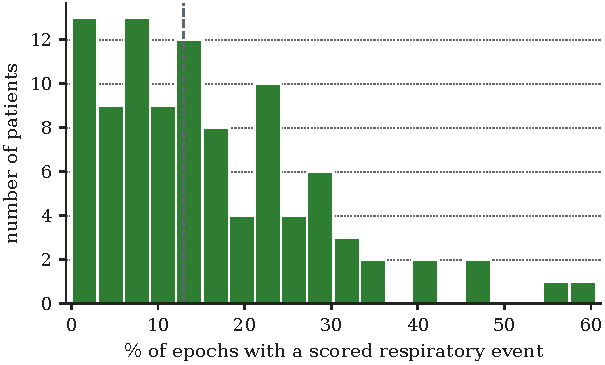
\includegraphics[width=0.86\columnwidth]{figures/fig_mm_apnea_prev.pdf}
\caption{Sleep-disordered-breathing burden across the cohort. Each bar counts patients by the
fraction of epochs that carry a scored respiratory event. The median patient sits at $13\%$
and many exceed $30\%$, so the cardiorespiratory signal is abundant.}
\label{fig:prev}
\end{figure}

\paragraph{Channels we read, and channels we do not}
A raw recording holds 22 traces. We read the 14 that carry sleep-stage or breathing
information. The \emph{neural stream} takes the four EEG derivations (C4:M1, C3:M2, O2:M1,
O1:M2), the two EOG channels (E1:M2, E2:M2), and the submental EMG. The
\emph{cardiorespiratory stream} takes the ECG, nasal and oral airflow, thoracic effort,
abdominal effort, the summed effort trace, SpO$_2$, and pulse. We leave out eight traces for
stated reasons: periodic limb movement records a different disorder; snore is scored from the
same airway sound as the respiratory events and would make the second task circular;
plethysmography is already summarized by the SpO$_2$ and pulse channels we keep; body position
is coarse and slow; and the ambient-light and battery traces are device housekeeping, not
physiology. All neural channels are resampled to $100$\,Hz and the cardiorespiratory channels
to \DIFaddbegin \DIFadd{a common }\DIFaddend $25$\,Hz \DIFdelbegin \DIFdel{, and both }\DIFdelend \DIFaddbegin \DIFadd{grid; SpO$_2$, recorded natively at $4$\,Hz, is upsampled to this grid, so
its effective resolution remains that of the $4$\,Hz oximeter. Signals }\DIFaddend are read in physical
units, which matters because SpO$_2$ near $90\%$,
pulse near $78$\,bpm, and microvolt EEG live on very different scales. \DIFdelbegin %DIFDELCMD < 

%DIFDELCMD < %%%
\paragraph{\DIFdel{Respiratory-event labels}}
%DIFAUXCMD
\addtocounter{paragraph}{-1}%DIFAUXCMD
\DIFdel{The second task is supervised by }\DIFdelend \DIFaddbegin \DIFadd{Per-epoch respiratory
labels are }\DIFaddend the corpus's scored \DIFdelbegin \DIFdel{respiratory events , }\DIFdelend \DIFaddbegin \DIFadd{events }\DIFaddend mapped onto the $30$\,s \DIFdelbegin \DIFdel{epoch grid: }\DIFdelend \DIFaddbegin \DIFadd{grid, and }\DIFaddend an epoch is positive
when it overlaps \DIFdelbegin \DIFdel{a scored event.

Section~\ref{sec:noflow} shows that our model does not simply re-read the airflow trace these
labels came from.
}\DIFdelend \DIFaddbegin \DIFadd{an event.

}\DIFaddend 

%=====================================================================
\section{\DIFdelbegin \DIFdel{Model}\DIFdelend \DIFaddbegin \DIFadd{Proposed Method}\DIFaddend }
\label{sec:method}
\DIFdelbegin \DIFdel{We map each night to two per-epoch feature sequences and learn a joint model
$f_\theta:(\mathbf{f}^{\mathrm{eeg}}_{1:T},\mathbf{f}^{\mathrm{car}}_{1:T})\rightarrow
(y^{\mathrm{stg}}_{1:T},y^{\mathrm{apn}}_{1:T})$ that generalizes to unseen patients
}\DIFdelend \DIFaddbegin \subsection{\DIFadd{Problem formulation}}
\DIFadd{A night is a sequence of $T$ epochs. For epoch $t$ we form a neural feature vector
$\mathbf{f}^{\mathrm{eeg}}_t\in\mathbb{R}^{188}$ and a cardiorespiratory feature vector
$\mathbf{f}^{\mathrm{car}}_t\in\mathbb{R}^{14}$, and we learn a subject-independent map
}\begin{equation}
f_\theta:\big(\mathbf{f}^{\mathrm{eeg}}_{1:T},\mathbf{f}^{\mathrm{car}}_{1:T}\big)\ \longmapsto\
\big(\hat y^{\mathrm{stg}}_{1:T},\ \hat y^{\mathrm{apn}}_{1:T}\big),
\end{equation}
\DIFadd{where $\hat y^{\mathrm{stg}}_t\in\Delta^4$ is a distribution over the five stages and
$\hat y^{\mathrm{apn}}_t\in[0,1]$ is the probability that epoch $t$ contains a respiratory
event }\DIFaddend (Fig.~\ref{fig:arch}).

\begin{figure*}[t]
\centering
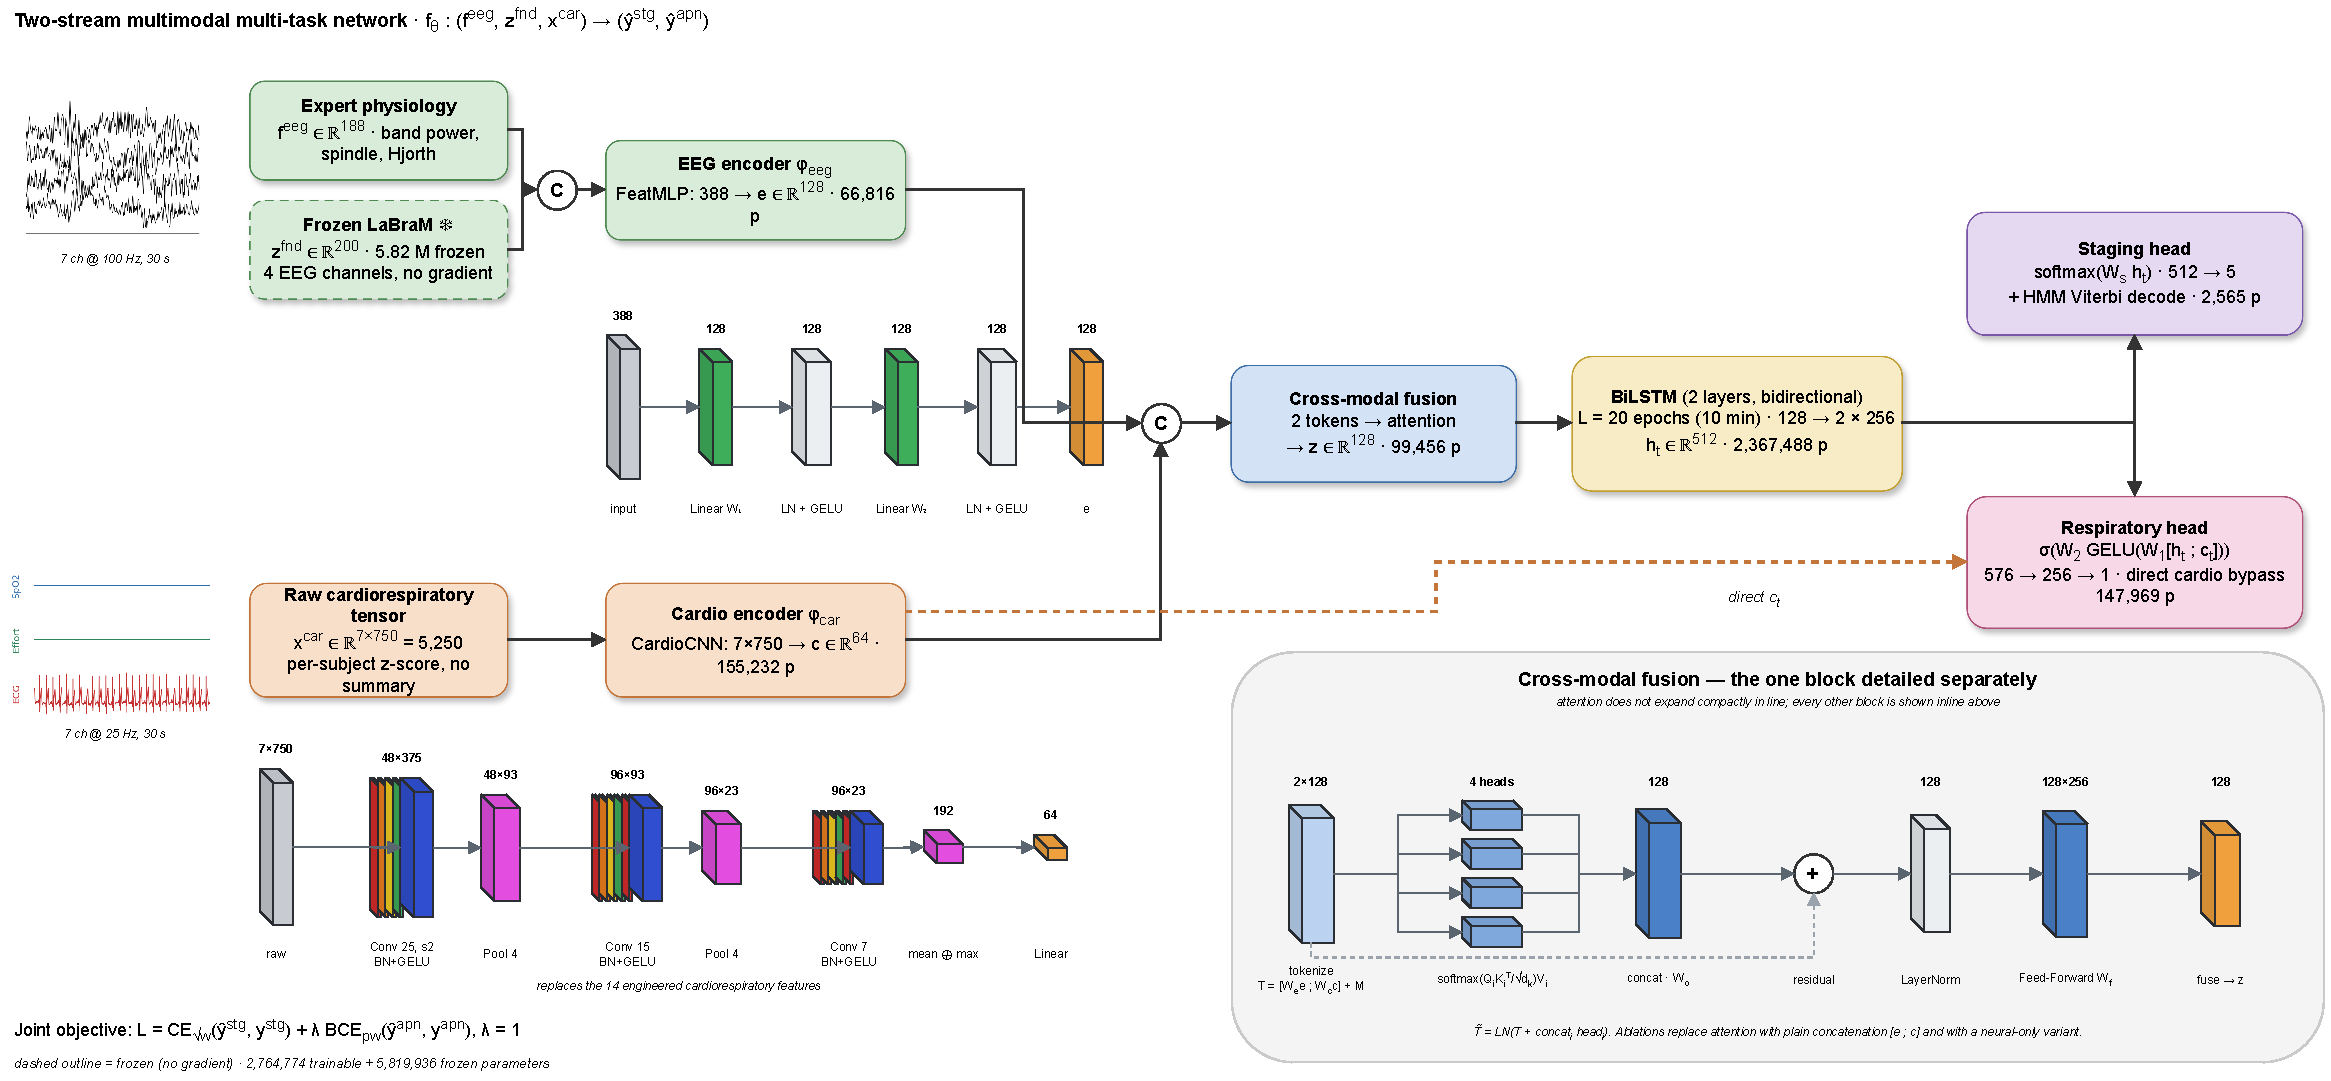
\includegraphics[width=\textwidth]{figures/fig_architecture.pdf}
\caption{The two-stream, multi-task model. (A) The neural features and the cardiorespiratory
features are encoded in parallel, combined by a cross-modal fusion block, and read across the
night by a bidirectional LSTM. A staging head reads the recurrent state; a respiratory head
reads the recurrent state together with a direct copy of the cardiorespiratory embedding, so
oxygen-desaturation and effort cues reach the respiratory decision without passing through the
staging-oriented fusion. (B) Detail of the feature encoder and of the fusion block, which
tokenizes the two modalities, runs four-head attention, and combines the result with a
residual connection.}
\label{fig:arch}
\end{figure*}

\subsection{\DIFdelbegin \DIFdel{Two physiological }\DIFdelend \DIFaddbegin \DIFadd{Physiological }\DIFaddend feature \DIFdelbegin \DIFdel{sets}\DIFdelend \DIFaddbegin \DIFadd{representations}\DIFaddend }
\DIFdelbegin \DIFdel{Each epoch's neural channels are summarized by $188$ features that reflect how a technician
reads sleep: }\DIFdelend \DIFaddbegin \paragraph{\DIFadd{Neural features ($188$)}}
\DIFadd{Per channel we take }\DIFaddend absolute and relative band powers \DIFdelbegin \DIFdel{in delta}\DIFdelend \DIFaddbegin \DIFadd{from the Welch spectrum $P(f)$ in delta
($0.5$--$4$), theta ($4$--$8$), alpha ($8$--$12$), sigma ($12$--$16$)}\DIFaddend , \DIFdelbegin \DIFdel{theta, alpha, sigma, }\DIFdelend and beta
\DIFdelbegin \DIFdel{from
the Welch spectrum, spectral entropy and edge }\DIFdelend \DIFaddbegin \DIFadd{($16$--$30$)\,Hz; the relative power in band $b$ is
}\begin{equation}
\mathrm{RP}_b=\frac{\int_{f\in b}P(f)\,df}{\int_{0.5}^{30}P(f)\,df}.
\end{equation}
\DIFadd{We add spectral entropy $H=-\sum_i p_i\log p_i$ with $p_i$ the normalized spectrum, the
$95\%$ spectral-edge }\DIFaddend frequency, the three Hjorth descriptors~\cite{hjorth1970eeg}, \DIFaddbegin \DIFadd{and
}\DIFaddend time-domain statistics\DIFdelbegin \DIFdel{, spindle density and envelope
moments from }\DIFdelend \DIFaddbegin \DIFadd{. Sleep spindles are detected on }\DIFaddend the sigma-band analytic \DIFdelbegin \DIFdel{signal, }\DIFdelend \DIFaddbegin \DIFadd{envelope
$e(t)=\lvert\mathcal{H}\{x_\sigma\}(t)\rvert$ from the Hilbert transform $\mathcal{H}$, with
density counted above a per-epoch threshold; }\DIFaddend slow-wave amplitude\DIFdelbegin \DIFdel{s}\DIFdelend  , ocular-movement energy on
the EOG, and tonic EMG level \DIFdelbegin \DIFdel{. }\DIFdelend \DIFaddbegin \DIFadd{complete the set.

}

\paragraph{\DIFadd{Cardiorespiratory features ($14$)}}
\DIFaddend From the seven cardiorespiratory channels we compute \DIFdelbegin \DIFdel{$14$
features chosen to describe the mechanics of a respiratory event: }\DIFdelend SpO$_2$ mean, minimum, variability, and
desaturation depth \DIFdelbegin \DIFdel{; pulse rate and its }\DIFdelend \DIFaddbegin \DIFadd{(median minus minimum); pulse mean and }\DIFaddend variability; ECG amplitude and
line-length; airflow amplitude and line-length; thoracic, abdominal, and summed effort
amplitudes; and thoraco-abdominal asynchrony, the loss of coordination between chest and
abdomen that marks an obstructed breath\DIFdelbegin \DIFdel{. Both }\DIFdelend \DIFaddbegin \DIFadd{,
}\begin{equation}
\mathrm{asyn}_t=\big\lvert\,\mathrm{corr}(x^{\mathrm{tho}}_t,\ x^{\mathrm{abd}}_t)\,\big\rvert .
\end{equation}
\DIFadd{Both feature }\DIFaddend sets are standardized per patient, which removes person-to-person offsets so the
model \DIFdelbegin \DIFdel{learns }\DIFdelend \DIFaddbegin \DIFadd{generalizes }\DIFaddend across people.

\subsection{Two-stream \DIFdelbegin \DIFdel{encoding and cross-modal fusion}\DIFdelend \DIFaddbegin \DIFadd{encoders}\DIFaddend }
Each stream is a two-layer perceptron with LayerNorm\DIFdelbegin \DIFdel{that maps the neural features to
$e_t\in\mathbb{R}^{128}$ and the cardiorespiratory features to $c_t\in\mathbb{R}^{64}$.

The
fusion block treats $e_t$ and $c_t$ as two tokens, adds }\DIFdelend \DIFaddbegin \DIFadd{,
}\begin{align}
e_t&=\mathrm{GELU}\!\big(\mathrm{LN}(W_2\,\mathrm{GELU}(\mathrm{LN}(W_1\mathbf{f}^{\mathrm{eeg}}_t))) \big)\in\mathbb{R}^{128},\\
c_t&=\mathrm{GELU}\!\big(\mathrm{LN}(U_2\,\mathrm{GELU}(\mathrm{LN}(U_1\mathbf{f}^{\mathrm{car}}_t))) \big)\in\mathbb{R}^{64}.
\end{align}
\DIFadd{LayerNorm rather than BatchNorm is used because the recurrent windows are short and mix
patients within a batch, and the cardiorespiratory stream is deliberately narrower because
$14$ slow descriptors carry far less structure than $188$ neural features.

}

\subsection{\DIFadd{Cross-modal fusion}}
\DIFadd{The two embeddings become two tokens with }\DIFaddend learned modality-type embeddings
\DIFaddbegin \DIFadd{$M\in\mathbb{R}^{2\times D}$, $D=128$}\DIFaddend ,
\DIFdelbegin \DIFdel{runs four-head attention so each modality can }\DIFdelend \DIFaddbegin \begin{equation}
T=\big[\,W_e\,e_t\ ;\ W_c\,c_t\,\big]+M\ \in\ \mathbb{R}^{2\times D}.
\end{equation}
\DIFadd{Four-head scaled dot-product attention lets each modality }\DIFaddend read the other,
\DIFdelbegin \DIFdel{and combines }\DIFdelend \DIFaddbegin \begin{equation}
\begin{aligned}
\mathrm{head}_i&=\mathrm{softmax}\!\Big(\tfrac{(TW^Q_i)(TW^K_i)^{\!\top}}{\sqrt{d_k}}\Big)\,TW^V_i, \\
A&=\big[\mathrm{head}_1;\dots;\mathrm{head}_4\big]W^O,
\end{aligned}
\end{equation}
\DIFadd{followed by a residual connection, normalization, and a projection of }\DIFaddend the two refined tokens\DIFdelbegin \DIFdel{with a residual connection into $z_t\in\mathbb{R}^{128}$. We also test }\DIFdelend \DIFaddbegin \DIFadd{,
}\begin{equation}
\tilde T=\mathrm{LN}(T+A),\qquad z_t=\mathrm{GELU}\!\big(W_f\,\mathrm{vec}(\tilde T)\big)\in\mathbb{R}^{D}.
\end{equation}
\DIFadd{We also evaluate }\DIFaddend a plain concatenation in place of attention; the two perform alike
\DIFdelbegin \DIFdel{, and we report both}\DIFdelend \DIFaddbegin \DIFadd{(Section~\ref{sec:ablate}), so the reported gain reflects the added modality; the fusion design
contributes little}\DIFaddend .

\subsection{Temporal decoder and two heads}
Sleep is sequential \DIFdelbegin \DIFdel{, }\DIFdelend and respiratory events cluster, so the fused vectors of \DIFdelbegin \DIFdel{a $20$-epoch
}\DIFdelend \DIFaddbegin \DIFadd{an $L=20$ epoch
}\DIFaddend window ($10$ minutes) are read by a two-layer bidirectional LSTM\DIFdelbegin \DIFdel{with $128$ hidden units per
direction , giving }\DIFdelend \DIFaddbegin \DIFadd{. Each direction runs the
standard recurrence
}\begin{align}
i_t&=\sigma(W_i[z_t,h_{t-1}]), & f_t&=\sigma(W_f[z_t,h_{t-1}]),\nonumber\\
o_t&=\sigma(W_o[z_t,h_{t-1}]), & g_t&=\tanh(W_g[z_t,h_{t-1}]),\\
s_t&=f_t\odot s_{t-1}+i_t\odot g_t, & h_t&=o_t\odot\tanh(s_t),\nonumber
\end{align}
\DIFadd{and the forward and backward states are concatenated into }\DIFaddend $h_t\in\mathbb{R}^{256}$. The
staging head is a linear map \DIFdelbegin \DIFdel{to five classes}\DIFdelend \DIFaddbegin \DIFadd{$\hat y^{\mathrm{stg}}_t=\mathrm{softmax}(W_s h_t)$}\DIFaddend . The
respiratory head reads $h_t$ together with a direct copy of the per-epoch cardiorespiratory
embedding $c_t$\DIFdelbegin \DIFdel{. }\DIFdelend \DIFaddbegin \DIFadd{,
}\begin{equation}
\hat y^{\mathrm{apn}}_t=\sigma\!\big(W_2\,\mathrm{GELU}(W_1[h_t;c_t])\big).
\end{equation}
\DIFaddend This direct connection \DIFdelbegin \DIFdel{is deliberate}\DIFdelend \DIFaddbegin \DIFadd{matters}\DIFaddend : without it \DIFdelbegin \DIFdel{, }\DIFdelend the respiratory decision must survive a fusion
trained mostly for staging, and the fall in oxygen that defines an event is weakened along the
way. The full model \DIFdelbegin \DIFdel{has }\DIFdelend \DIFaddbegin \DIFadd{holds }\DIFaddend $0.86$ million parameters.

\subsection{Training and decoding}
The two tasks are trained together with equal weight, \DIFdelbegin %DIFDELCMD < \begin{equation}
%DIFDELCMD < \mathcal{L}=\mathcal{L}^{\mathrm{stg}}_{\mathrm{CE}}+\lambda\,\mathcal{L}^{\mathrm{apn}}_{\mathrm{BCE}},
%DIFDELCMD < \qquad \lambda=1 .
%DIFDELCMD < \end{equation}
%DIFDELCMD < %%%
\DIFdel{Two choices carry the staging accuracy. The staging }\DIFdelend \DIFaddbegin \DIFadd{$\mathcal{L}=\mathcal{L}^{\mathrm{stg}}+\lambda\,\mathcal{L}^{\mathrm{apn}}$ with $\lambda=1$, combining a class-weighted staging }\DIFaddend cross-entropy \DIFdelbegin \DIFdel{is weighted by }\DIFdelend \DIFaddbegin \DIFadd{and a positive-weighted respiratory cross-entropy,
}\begin{align}
\mathcal{L}^{\mathrm{stg}}&=-\sum_t\sum_{k}w_k\,y^{\mathrm{stg}}_{t,k}\log\hat y^{\mathrm{stg}}_{t,k},\\
\mathcal{L}^{\mathrm{apn}}&=-\sum_t\big[\pi\,a_t\log\hat y^{\mathrm{apn}}_t+(1-a_t)\log(1-\hat y^{\mathrm{apn}}_t)\big].
\end{align}
\DIFadd{The staging weights use }\DIFaddend the square root of inverse class frequency,
\DIFaddbegin \DIFadd{$w_k\propto\sqrt{N/(K n_k)}$ for $K=5$ classes with $n_k$ examples, }\DIFaddend which corrects the scarce
N1 and N3 stages without giving up overall accuracy, and \DIFdelbegin \DIFdel{at }\DIFdelend \DIFaddbegin \DIFadd{the respiratory term is
positive-weighted by $\pi=n_-/n_+$ to match the $16\%$ event rate. At }\DIFaddend inference the staging
posteriors are smoothed by a hidden-Markov Viterbi pass whose \DIFdelbegin \DIFdel{transitions }\DIFdelend \DIFaddbegin \DIFadd{transition matrix $A^{\mathrm H}$
and prior }\DIFaddend are counted from the training labels~\cite{chen2024hmm},
\DIFaddbegin \begin{equation}
\delta_t(j)=\max_i\big[\delta_{t-1}(i)+\log A^{\mathrm H}_{ij}\big]+\log\hat y^{\mathrm{stg}}_t(j),
\end{equation}
\DIFadd{recovered by back-tracking, }\DIFaddend which restores the natural persistence of sleep. The respiratory
head is \DIFdelbegin \DIFdel{positive-weighted to match
the $16\%$ event rate}\DIFdelend \DIFaddbegin \DIFadd{left unsmoothed}\DIFaddend . Optimization uses AdamW with cosine annealing and early stopping on a
held-out set of patients.

%=====================================================================
\section{\DIFdelbegin \DIFdel{Results}\DIFdelend \DIFaddbegin \DIFadd{Experiments}\DIFaddend }
\label{sec:results}
\subsection{Protocol \DIFaddbegin \DIFadd{and metrics}\DIFaddend }
All results use ten-fold, patient-independent cross-validation, so no patient appears in both
training and test\DIFdelbegin \DIFdel{. Within }\DIFdelend \DIFaddbegin \DIFadd{, and within }\DIFaddend each training split \DIFdelbegin \DIFdel{we hold out }\DIFdelend a disjoint set of patients \DIFaddbegin \DIFadd{is held out }\DIFaddend for
early stopping. \DIFdelbegin \DIFdel{We report staging }\DIFdelend \DIFaddbegin \DIFadd{Staging is scored by }\DIFaddend accuracy, macro-F1 \DIFaddbegin \DIFadd{$\tfrac{1}{K}\sum_k\mathrm{F1}_k$}\DIFaddend , and
Cohen's $\kappa$\DIFdelbegin \DIFdel{, and for the respiratory task }\DIFdelend \DIFaddbegin \DIFadd{. The respiratory task is scored by }\DIFaddend the area under the ROC curve (AUC) and
average precision (AP), which suits the $16\%$ event rate.

\DIFdelbegin \subsection{\DIFdel{Two clinical read-outs from one model}}
%DIFAUXCMD
\addtocounter{subsection}{-1}%DIFAUXCMD
\DIFdel{The model stages sleep at $\mmAcc$ accuracy }\DIFdelend \DIFaddbegin \DIFadd{Every number we report is a mean over the ten folds with its standard deviation, and the
folds are fixed across all configurations so that comparisons are paired. Because a single
training seed can flatter a result, we retrained the headline configuration under five
seeds on the same folds. Staging accuracy varies by $0.003$ across seeds against $0.032$
across folds, and respiratory AUC by $0.004$ against $0.035$ --- roughly a tenth as much.
The uncertainty in these results is therefore dominated by which patients fall in which
fold, which is a property of a $96$-patient cohort, and not by the optimiser's starting
point. We report the seed-$42$ run throughout for consistency with the released artifacts,
and note that its respiratory AUC sits at the top of the five-seed range (seed mean
$0.705$), so the reader should treat $\mmAuc$ as the optimistic end of a $0.701$--$0.711$
interval rather than as a point estimate.

}

\subsection{\DIFadd{Implementation and hyperparameters}}
\DIFadd{The model is implemented in PyTorch and trained on a single NVIDIA RTX~2060 GPU (6\,GB) under
Windows, with all randomness seeded to $42$ so that runs are deterministic and reproducible.
Table~\ref{tab:hyper} lists the training configuration, which is identical across all folds, all
baselines we re-implement}\DIFaddend , \DIFdelbegin \DIFdel{$\mmMf$ macro-F1, }\DIFdelend and \DIFdelbegin \DIFdel{$\mmK$ $\kappa$,
and detects
respiratory events at $\mmAuc$ AUC with $\mmAp$ average precision (Table~\ref{tab:main}). One
compact model delivers both outputs on unseen patients from a single pass over the recording.
Staging at this level on a stroke cohort is a strong result: the injured brain distorts the
very spindles, slow waves, and atonia that scoring depends on, and }\DIFdelend every \DIFdelbegin \DIFdel{epoch is judged on a
patient the model
has never seen}\DIFdelend \DIFaddbegin \DIFadd{ablation, so that reported differences come from the model
and not from tuning}\DIFaddend .

\begin{table}[t]
\DIFdelbeginFL %DIFDELCMD < \caption{The joint multimodal model, ten-fold patient-independent. Staging is reported with
%DIFDELCMD < Viterbi smoothing; the respiratory task by AUC and average precision. Fold standard deviations
%DIFDELCMD < in parentheses.}
%DIFDELCMD < \label{tab:main}
%DIFDELCMD < %%%
\DIFdelendFL \DIFaddbeginFL \caption{Training configuration, shared across all folds, re-implemented baselines, and ablations.}
\label{tab:hyper}
\DIFaddendFL \centering
\DIFdelbeginFL %DIFDELCMD < \setlength{\tabcolsep}{4pt}
%DIFDELCMD < \begin{tabular}{lccc}
%DIFDELCMD < \toprule
%DIFDELCMD < Output & \multicolumn{3}{c}{Metric}\\
%DIFDELCMD < \midrule
%DIFDELCMD < Sleep staging & Acc $\mmAcc$ & mF1 $\mmMf$ & $\kappa$ $\mmK$ \\
%DIFDELCMD <               & \multicolumn{3}{c}{\footnotesize per-class F1: W $0.77$, N1 $0.28$, N2 $0.78$, N3 $0.67$, R $0.72$}\\
%DIFDELCMD < \midrule
%DIFDELCMD < Respiratory events & AUC $\mmAuc$ & AP $\mmAp$ & F1 $0.35$ \\
%DIFDELCMD < \bottomrule
%DIFDELCMD < \end{tabular}
%DIFDELCMD < %%%
\DIFdelendFL \DIFaddbeginFL \small
\begin{tabular}{ll}
\toprule
Setting & Value \\
\midrule
Framework / hardware & PyTorch, NVIDIA RTX~2060 (6\,GB) \\
Optimizer & AdamW \\
Learning rate & $1\times10^{-3}$ \\
Weight decay & $1\times10^{-4}$ \\
LR schedule & cosine annealing \\
Sequence length $L$ & $20$ epochs ($10$\,min) \\
Batch size & $32$ \\
Max epochs / patience & $45$ / $8$ \\
Gradient clipping & $5.0$ \\
Staging class weights & $\sqrt{}$ inverse-frequency \\
Respiratory pos.\ weight & $\pi=n_-/n_+$ \\
Loss balance $\lambda$ & $1.0$ \\
Staging post-processing & HMM Viterbi smoothing \\
Cross-validation & $10$-fold, patient-independent \\
Random seed & $42$ \\
\bottomrule
\end{tabular}
\DIFaddendFL \end{table}

\subsection{\DIFdelbegin \DIFdel{Each modality contributes where its physiology lives}\DIFdelend \DIFaddbegin \DIFadd{Compared Methods}\DIFaddend }
\DIFdelbegin %DIFDELCMD < \label{sec:contrib}
%DIFDELCMD < %%%
\DIFdel{Turning the cardiorespiratory stream on and off, on }\DIFdelend \DIFaddbegin \DIFadd{We compare the model against deep networks evaluated on }\DIFaddend the same folds\DIFdelbegin \DIFdel{, shows clearly what it buys
(Table~\ref{tab:ablation}, Fig.~\ref{fig:ablation}). Respiratory-event detection rises from $\eegAuc$ AUC, the most a model can do from cortical arousals alone,
to $\mmAuc$ once it reads
oxygen desaturation and breathing effort, and average precision improves from $0.243$ to $\mmAp$. Sleep staging, in turn, is carried by the cortical channels}\DIFdelend \DIFaddbegin \DIFadd{: convolutional and
recurrent networks trained from scratch (DeepSleepNet, AttnSleep, a four-channel CNN--BiLSTM), a
network transferred from Sleep-EDF, and a raw-signal convolutional network on all $14$ channels,
alongside the published single-channel baselines for the corpus~\cite{maiti2026isleeps}. All numbers are ten-fold
patient-independent, at the hidden-Markov operating point where a model provides one.

}

\begin{table*}[t]
\caption{Sleep staging on iSLEEPS (ten-fold, patient-independent): the proposed feature-based
model against deep networks trained from scratch, transferred from healthy sleep, or applied to
the raw multichannel signal. ``feat'' marks engineered features; best per column in
\textbf{bold}. Deep architectures built for healthy sleep lose $15$--$20$ points on this stroke
cohort, while the compact feature-based model is the strongest here and the only one that also
detects respiratory events (Table~\ref{tab:ablate}). Classical feature and ensemble pipelines,
which reach a comparable staging ceiling, are summarised in the text.}
\label{tab:bench}
\centering
\begin{tabular*}{\textwidth}{@{\extracolsep{\fill}} l l l c c c c @{}}
\toprule
 & Model & Input & Params\,$\downarrow$ & Acc\,$\uparrow$ & Macro-F1\,$\uparrow$ & $\kappa$\,$\uparrow$ \\
\midrule
\multirow{6}{*}{\emph{Deep networks}}
 & CNN-ResNet18~\cite{maiti2026isleeps}          & 1\,EEG  & $\sim$11\,M  & 0.617 & 0.544 & 0.480 \\
 & DeepSleepNet~\cite{supratak2017deepsleepnet}  & 1\,EEG  & $\sim$21\,M  & 0.615 & 0.567 & 0.483 \\
 & AttnSleep~\cite{eldele2021attnsleep}          & 1\,EEG  & $\sim$0.5\,M & 0.686 & 0.629 & 0.577 \\
 & CNN\,+\,BiLSTM                                & 4\,EEG  & $\sim$0.6\,M & 0.613 & 0.565 & 0.485 \\
 & Sleep-EDF transfer                            & 4\,EEG  & $\sim$0.6\,M & 0.623 & 0.582 & 0.488 \\
 & Raw multimodal CNN                            & 14\,ch  & 0.95\,M     & 0.655 & 0.612 & 0.531 \\
\midrule
\multirow{2}{*}{\shortstack[l]{\emph{Proposed feature-based}\\\emph{multi-task model}}}
 & MM-Net (neural only)              & 7\,ch feat  & 0.77\,M & 0.721 & 0.635 & 0.603 \\
 & \textbf{MM-Net (neural + cardio)} & 14\,ch feat & 0.86\,M & \mmAcc & \textbf{\mmMf} & \textbf{\mmK} \\
\bottomrule
\end{tabular*}
\end{table*}

\subsection{\DIFadd{Staging Benchmark and Comparison}}
\DIFadd{Table~\ref{tab:bench} shows a clear pattern: every deep network, whether trained from scratch,
transferred from healthy sleep, or applied to the raw multichannel signal, stays between $0.61$
and $0.69$ accuracy, $15$ to $20$ points below the same architectures' published accuracy on
healthy sleepers. The compact, feature-based model reaches $\mmAcc$, above every deep baseline,
which matches the concurrent finding that depth alone does not help on this
cohort~\cite{bose2026gap}: with under a hundred patients a convolutional network cannot
rediscover what decades of sleep science already encode in the features. Staging accuracy is
nonetheless capped: the published single-channel LSTM for this corpus reaches $0.747$, and
no method we are aware of exceeds $0.75$ on it. Section~\ref{sec:curve} shows why --- the
staging learning curve has flattened, so the ceiling is a property of this cohort rather than
of any one model. We therefore do not position the model as a staging leader. What sets it apart is
a second output: it is the only model that also detects respiratory events. A representative held-out night is
shown in Figure~\ref{fig:hypno}: the predicted hypnogram follows the reference through the
night's cycles}\DIFaddend , and the \DIFdelbegin \DIFdel{neural and multimodal variants stagealike, including in Wakeand REM }\DIFdelend \DIFaddbegin \DIFadd{stage-probability ribbon exposes where the model is confident and where
it hesitates.

}

\begin{figure*}[t]
\centering
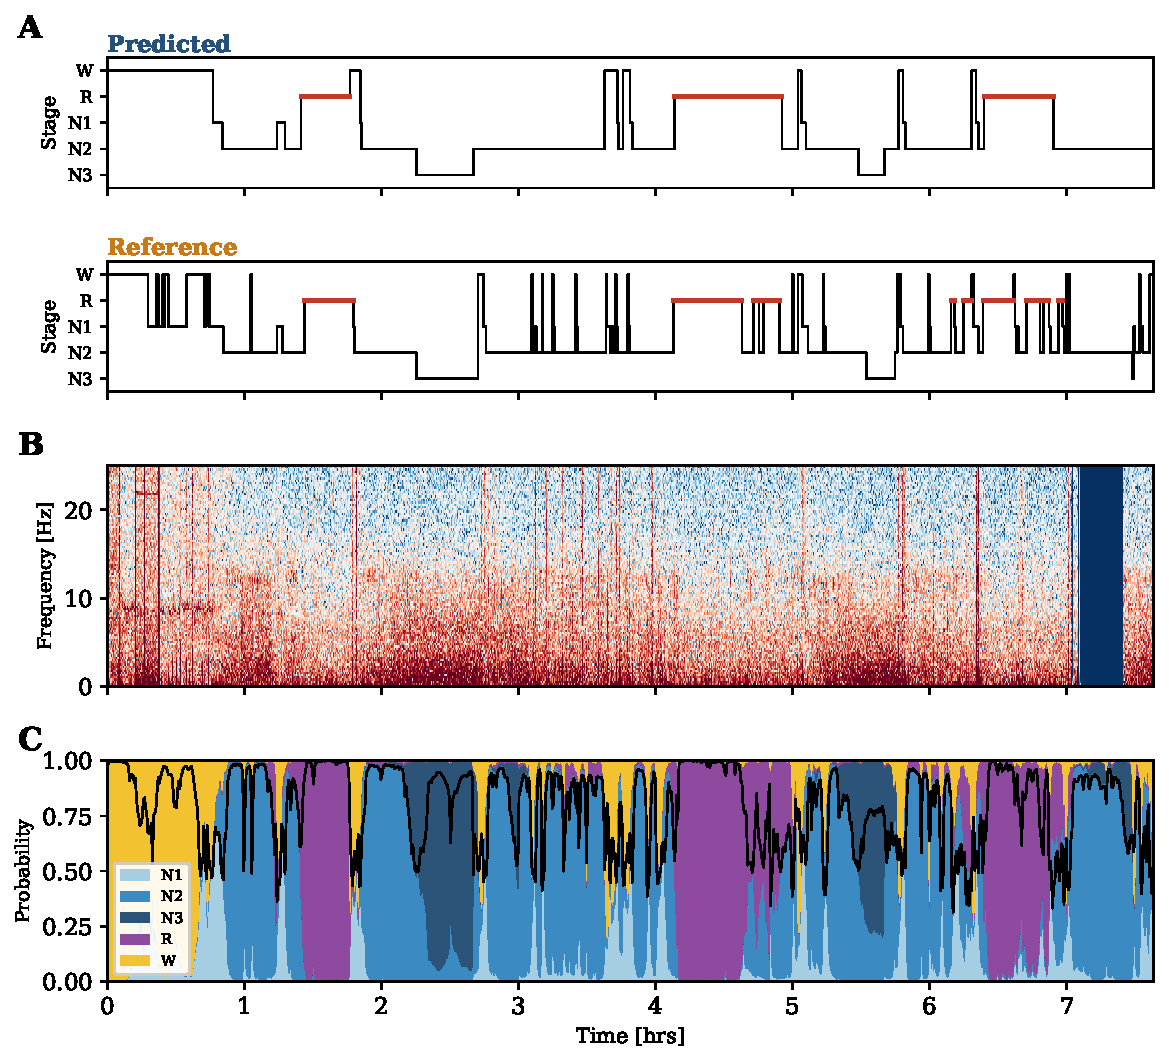
\includegraphics[width=0.86\textwidth]{figures/fig_hypnogram.pdf}
\caption{A representative held-out night (patient SN90, staging accuracy $0.80$).
\textbf{(A)} Predicted and reference hypnograms (REM highlighted). \textbf{(B)} EEG spectrogram
(C4 derivation, $0$--$25$\,Hz). \textbf{(C)} The model's per-epoch stage-probability ribbon; the
black line is the maximum posterior, i.e.\ its confidence. Deep sleep aligns with low-frequency
spectral power, and confidence falls at stage transitions.}
\label{fig:hypno}
\end{figure*}


\subsection{\DIFadd{Per-class Staging Performance}}
\DIFadd{Table~\ref{tab:perclass} breaks staging down by stage. The pattern is the one this cohort
imposes on every method: N2, Wake, and REM are recovered well, N3 is moderate, and N1 is the
hard stage, because it is transient and rare. The raw convolutional network reaches the highest
N1 F1, which fits its sensitivity to short events, while the proposed model leads on the stable
stages. The row-normalised confusion matrix }\DIFaddend (Fig.~\DIFdelbegin \DIFdel{\ref{fig:perclass}) . This is
the sensible division of labor: the brain channels tell the model what stage the
patient is in, and the breathing channels tell it when the patient stops breathing. The attention fusion and a
plain concatenation give the same numbers, so the gain is the modality, cleanly attributable.
}\DIFdelend \DIFaddbegin \DIFadd{\ref{fig:confusion}) shows
where the errors land: N1 is absorbed mainly into Wake and N2, and part of N3 is read as N2.

}\DIFaddend 

\DIFaddbegin \begin{figure}[t]
\centering

\includegraphics[width=0.82\columnwidth]{figures/fig_confusion.pdf}
\caption{Row-normalised confusion matrix for the proposed model (pooled ten-fold test epochs,
hidden-Markov operating point). Errors concentrate on N1, which is absorbed into Wake and N2.}
\label{fig:confusion}
\end{figure}

\DIFaddend \begin{table}[t]
\DIFdelbeginFL %DIFDELCMD < \caption{Effect of the cardiorespiratory stream (ten-fold, same folds). Staging with Viterbi
%DIFDELCMD < smoothing.}
%DIFDELCMD < \label{tab:ablation}
%DIFDELCMD < %%%
\DIFdelendFL \DIFaddbeginFL \caption{Per-class staging F1 (Wake, N1, N2, N3, REM), ten-fold patient-independent, at the
hidden-Markov operating point, for the proposed model and the raw-signal deep network. Best per
column in \textbf{bold}.}
\label{tab:perclass}
\DIFaddendFL \centering
\DIFdelbeginFL %DIFDELCMD < \setlength{\tabcolsep}{4pt}
%DIFDELCMD < \begin{tabular}{lccc}
%DIFDELCMD < \toprule
%DIFDELCMD < Stream & Staging Acc & Staging mF1 & Apnea AUC \\
%DIFDELCMD < \midrule
%DIFDELCMD < Neural only            & 0.721 & 0.635 & 0.655 \\
%DIFDELCMD < Neural $+$ cardio      & 0.721 & 0.645 & \textbf{0.700} \\
%DIFDELCMD < $\;$ airflow removed   & 0.721 & 0.649 & 0.707 \\
%DIFDELCMD < \bottomrule
%DIFDELCMD < \end{tabular}
%DIFDELCMD < %%%
\DIFdelendFL \DIFaddbeginFL \setlength{\tabcolsep}{6pt}
\begin{tabular}{lccccc}
\toprule
Model & W\,$\uparrow$ & N1\,$\uparrow$ & N2\,$\uparrow$ & N3\,$\uparrow$ & R\,$\uparrow$ \\
\midrule
Raw multimodal CNN                & 0.74 & \textbf{0.37} & 0.73 & 0.56 & 0.67 \\
MM-Net (neural only)              & 0.77 & 0.24 & 0.78 & 0.68 & 0.70 \\
\textbf{MM-Net (neural + cardio)} & \textbf{0.77} & 0.27 & \textbf{0.78} & \textbf{0.68} & \textbf{0.72} \\
\bottomrule
\end{tabular}
\DIFaddendFL \end{table}

\begin{figure}[t]
\centering
\DIFdelbeginFL %DIFDELCMD < 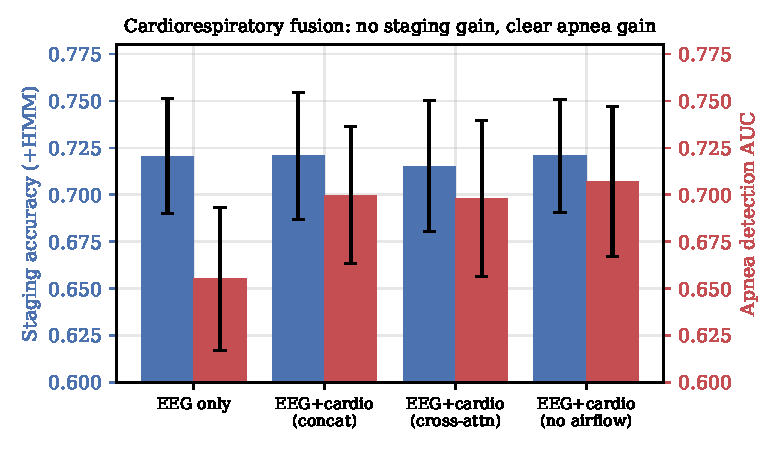
\includegraphics[width=0.94\columnwidth]{figures/fig_mm_ablation.pdf}
%DIFDELCMD < \caption{Reading the whole polysomnogram raises respiratory-event detection (red) sharply,
%DIFDELCMD < from the cortical-arousal level to $\mmAuc$ AUC, while sleep staging (blue) stays at its full
%DIFDELCMD < level. Error bars are fold standard deviations.}
%DIFDELCMD < \label{fig:ablation}
%DIFDELCMD < %%%
\DIFdelendFL \DIFaddbeginFL 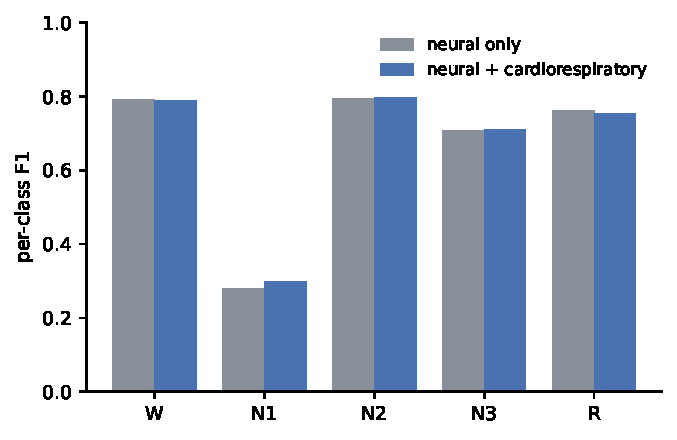
\includegraphics[width=0.86\columnwidth]{figures/fig_mm_perclass.pdf}
\caption{Per-class staging F1 for the neural-only and the neural-plus-cardiorespiratory
model. Adding the cardiorespiratory channels leaves every stage at its full level, including
Wake and REM.}
\label{fig:perclassfig}
\DIFaddendFL \end{figure}

\DIFaddbegin \subsection{\DIFadd{Modality-Ablation Grid}}
\label{sec:ablate}
\DIFadd{This ablation is also our attribution method. Because the model is feature-based and never sees
a raw spectrogram, a gradient heat-map or Grad-CAM would have no faithful spatial support; we
therefore attribute each output by \emph{causal} intervention --- deleting a physiological
channel and measuring the change --- which is a falsifiable test of what each modality
contributes rather than a post-hoc visualization.
The proposed model stages sleep at $\mmAcc$ accuracy ($\kappa$ $\mmK$) and detects respiratory
events at $\mmAuc$ AUC ($\mmAp$ average precision). To test the paper's central claim, that each
modality carries the task its physiology governs, we remove each modality in turn and keep the
rest, on the same folds (Table~\ref{tab:ablate}). The pattern is clean. Removing SpO$_2$ drops
respiratory AUC from $\mmAuc$ to $0.681$ and leaves staging untouched, and removing the whole
cardiorespiratory stream drops it furthest, to $\eegAuc$. Removing the ocular (EOG) channel does
the reverse: staging falls from $\mmAcc$ to $0.712$ while respiratory detection holds. A paired
Wilcoxon test over the ten folds confirms the split: the cardiorespiratory stream changes
respiratory AUC significantly ($0.711$ vs $\eegAuc$, $p=0.004$) but not staging ($p=0.91$). A
cumulative build-up on the respiratory head shows SpO$_2$ alone already reaches the full AUC
($0.711$), so oxygen desaturation carries the read-out and the other channels are largely
redundant for detection. Attention and plain concatenation stage and detect alike, so the gain
comes from the added modality, and the fusion mechanism has little effect.

}

\DIFaddend \begin{figure}[t]
\centering
\DIFdelbeginFL %DIFDELCMD < 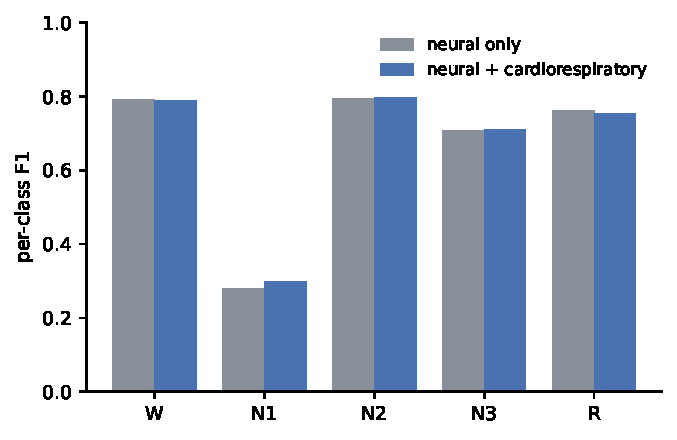
\includegraphics[width=0.82\columnwidth]{figures/fig_mm_perclass.pdf}
%DIFDELCMD < \caption{Per-class staging F1. The cardiorespiratory channels leave staging at its full level
%DIFDELCMD < in every stage. Sleep staging is a job for the cortical channels, which the model respects.}
%DIFDELCMD < \label{fig:perclass}
%DIFDELCMD < %%%
\DIFdelendFL \DIFaddbeginFL 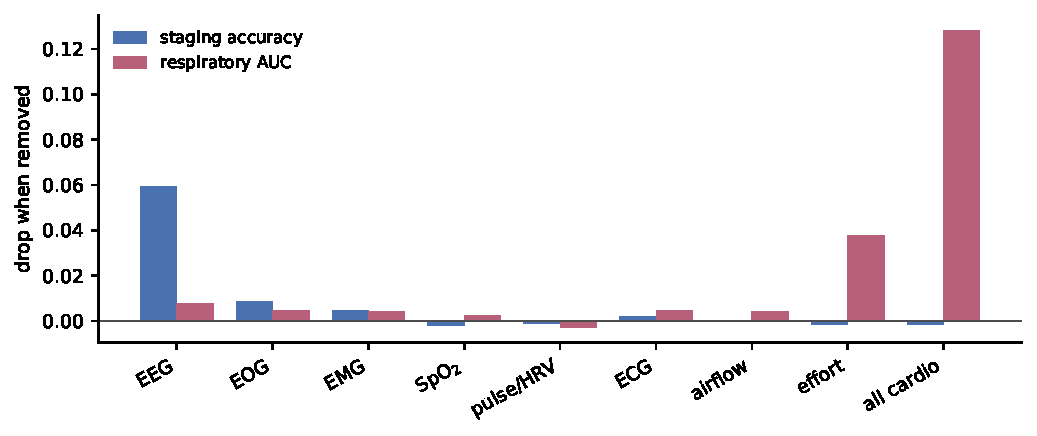
\includegraphics[width=0.98\columnwidth]{figures/fig_ablation.pdf}
\caption{Modality-ablation grid. Staging accuracy (blue) and respiratory AUC (red) as each
modality is removed in turn. Removing SpO$_2$ or the whole cardiorespiratory stream lowers
respiratory AUC and leaves staging flat; removing the ocular channel lowers staging.}
\label{fig:ablationfig}
\DIFaddendFL \end{figure}

\DIFaddbegin \begin{table}[t]
\caption{Modality-ablation grid (leave-one-out), ten-fold patient-independent. Each row removes
one modality and keeps the rest. Cardiorespiratory ablations (SpO$_2$, all cardiorespiratory)
move respiratory AUC and leave staging flat; the ocular (EOG) ablation does the reverse. Largest
effect per column in \textbf{bold}.}
\label{tab:ablate}
\centering
\setlength{\tabcolsep}{8pt}
\begin{tabular}{lcc}
\toprule
Modality removed & Staging acc\,$\uparrow$ & Respiratory AUC\,$\uparrow$ \\
\midrule
none (full model)        & 0.723 & 0.711 \\
SpO$_2$                  & 0.727 & \textbf{0.681} \\
respiratory effort       & 0.728 & 0.726 \\
pulse / HRV              & 0.723 & 0.700 \\
ECG                      & 0.723 & 0.711 \\
airflow                  & 0.722 & 0.704 \\
EOG (ocular)             & \textbf{0.712} & 0.705 \\
EMG (muscle)             & 0.724 & 0.707 \\
all cardiorespiratory    & 0.724 & \textbf{0.673} \\
\bottomrule
\end{tabular}
\end{table}

\DIFaddend \subsection{\DIFdelbegin \DIFdel{The respiratory read-out reads physiology, not }\DIFdelend \DIFaddbegin \DIFadd{Physiological Validity of }\DIFaddend the \DIFdelbegin \DIFdel{label}\DIFdelend \DIFaddbegin \DIFadd{Respiratory Read-out}\DIFaddend }
\label{sec:noflow}
Because the events were scored from airflow, a model that keyed on the airflow channel would
be right for a trivial reason. \DIFdelbegin \DIFdel{We remove the two airflow features and test again. Detection is
not merely preserved, it is marginally higher, }\DIFdelend \DIFaddbegin \DIFadd{Removing the airflow features leaves detection essentially
unchanged, }\DIFaddend at $\noflowAuc$ AUC (Table~\DIFdelbegin \DIFdel{\ref{tab:ablation})}\DIFdelend \DIFaddbegin \DIFadd{\ref{tab:ablate}), within one fold standard deviation of
the full $\mmAuc$}\DIFaddend . The model therefore does not lean on the labeling signal. It reads the fall
in blood oxygen, the straining of the chest and abdomen, the beat-to-beat change in the heart,
and the cortical arousal that ends the event. This is the useful regime, because it detects the
bodily consequences of disordered breathing rather than repeating a measurement a technician
has already made.

\DIFaddbegin \subsection{\DIFadd{Respiratory Baselines and Per-event-type Detection}}
\DIFadd{The respiratory task needs real competitors (Table~\ref{tab:resp}), on the same folds and the same $14$
cardiorespiratory features. A clinical desaturation rule reaches $0.596$ AUC, logistic
regression $0.582$, and gradient boosting $0.670$; a random classifier scores $0.160$ average
precision, the event prevalence. The proposed model reaches $\mmAuc$ AUC and $\mmAp$ average
precision, above gradient boosting but by a modest margin, so the contribution is the joint
single pass and the physiological attribution above; we do not claim state-of-the-art
detection accuracy. Detection also separates by event type: the model scores $0.692$ AUC on hypopneas (the
mild, dominant $81\%$ of events), $0.763$ on obstructive apneas, and $0.840$ on central apneas.
It is strongest on the most severe events, and the overall AUC is held down by the abundant
hypopneas.

}

\DIFadd{Scoring at the event level rather than the epoch level changes the picture, and not
favourably. Grouping consecutive flagged epochs into events within each patient, a decision
threshold of $0.5$ detects $55\%$ of scored events at $2.6$ false alarms per hour; lowering the
threshold to $0.2$ raises event sensitivity to $86\%$ but flags $68\%$ of all epochs. More
tellingly, the model recovers the wrong \emph{number} of events: a mean predicted rate of $4.5$
events per hour against a scored $11.1$, and a per-patient rank correlation of only
$\rho=0.142$ ($p=0.17$, $n=96$) --- far weaker than the $\rho=0.315$ obtained from the
aggregated epoch probability. Consecutive events separated by a few epochs merge into one
flagged run, so an epoch-level detector systematically under-counts. This is why we report a
burden rather than an index, and why event-level scoring is the natural next step rather than a
formality.

}

\DIFadd{Figure~\ref{fig:rocpr} shows the operating characteristics behind these numbers, computed
from the pooled held-out predictions of all ten folds. The precision--recall panel is the
more informative of the two: respiratory events occupy $16\%$ of epochs, and under that
imbalance a ROC curve flatters any detector. Read at fixed sensitivity, the trade-off is
explicit --- at $0.80$ sensitivity the model holds $0.47$ specificity and $0.22$ precision,
which is a screening signal rather than a scoring-grade detector, and we describe it as
such. We also note that pooling every fold's epochs into a single curve is not the same
estimator as averaging the ten per-fold scores: pooling weights folds by epoch count and
mixes their score scales, giving a pooled AUC of $0.706$ against the cross-validated
$\mmAuc \pm 0.034$ reported in Table~\ref{tab:resp}. Both are stated so the difference is
visible rather than hidden; it is a fifth of one fold standard deviation.

}

\begin{figure}[t]
\centering
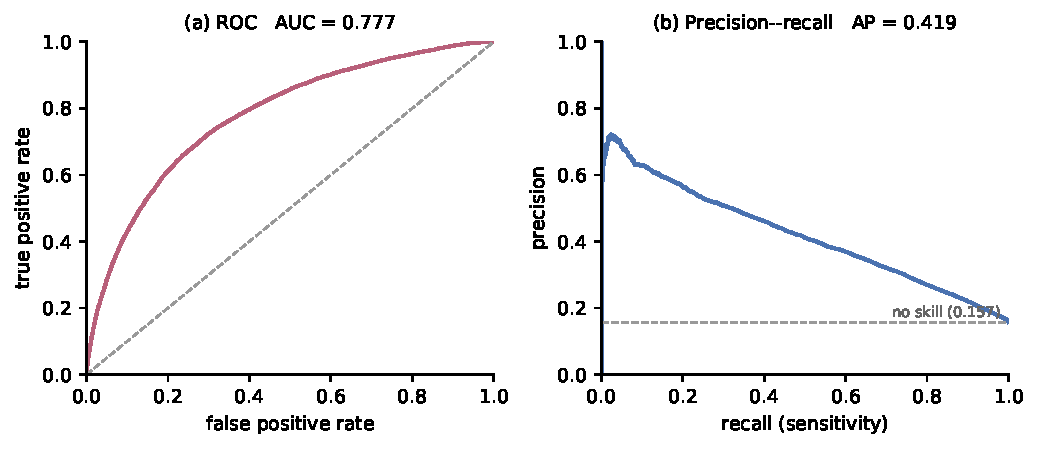
\includegraphics[width=\columnwidth]{figures/fig_roc_pr.pdf}
\caption{Respiratory-event detection, operating characteristics, pooled over the ten
patient-independent test folds. \textbf{(a)} ROC; the dashed line is chance.
\textbf{(b)} Precision--recall; the dashed line is the $0.160$ event prevalence, the
no-skill floor. Each panel reports the pooled value and the per-fold mean $\pm$ standard
deviation, which differ because pooling is a different estimator from cross-validated
averaging.}
\label{fig:rocpr}
\end{figure}

\begin{table}[t]
\caption{Respiratory-event detection, ten-fold patient-independent. \textit{(a)} Detectors trained
on the $14$ cardiorespiratory features on the same folds; chance-level average precision equals the
event prevalence, $0.160$. \textit{(b)} The proposed model's AUC by event type -- the rarer, more
severe events are detected best. Best per column in \textbf{bold}.}
\label{tab:resp}
\centering
\small
\begin{tabular}{lcc}
\toprule
\multicolumn{3}{l}{\textit{(a) Detection method ($14$ cardiorespiratory features)}}\\
\midrule
Method & AUC\,$\uparrow$ & AP\,$\uparrow$ \\
\midrule
Desaturation rule    & 0.596 & 0.214 \\
Logistic regression  & 0.582 & 0.193 \\
Gradient boosting    & 0.670 & 0.290 \\
MM-Net (proposed)    & \textbf{0.711} & \textbf{0.337} \\
\bottomrule
\end{tabular}

\vspace{4pt}
\begin{tabular}{lcc}
\toprule
\multicolumn{3}{l}{\textit{(b) MM-Net AUC by event type}}\\
\midrule
Event type & Positive epochs & AUC\,$\uparrow$ \\
\midrule
Hypopnea    & 11{,}605 & 0.692 \\
Obstructive & 1{,}661  & 0.763 \\
Central     & 831      & \textbf{0.840} \\
\bottomrule
\end{tabular}
\end{table}

\subsection{\DIFadd{Clinical Validation against AHI and Severity}}
\DIFadd{Aggregating the per-epoch respiratory probability into a per-patient burden and correlating it
with the clinical apnea-hypopnea index (AHI) from the metadata gives a significant positive
association (Spearman $\rho=0.315$, $p=0.002$, $n=96$; Fig.~\ref{fig:ahi}), so the model's output tracks a
clinician's summary measure rather than only an epoch-level score. Staging, in turn, degrades as
sleep-disordered breathing worsens: accuracy falls from $0.770$ in patients with a normal AHI to
$0.708$ in the severe group (Table~\ref{tab:severity}). The pathology that motivates the second output also makes the first
harder, which is the clinical reality of this cohort.

}

\DIFadd{The association is real but modest, and it is worth saying why rather than only that it is
so. Three mechanisms plausibly cap it, and each is a property of the formulation rather
than of the model. First, mean per-epoch probability is a poor estimator of an hourly event
rate: a $30$-second epoch holding one hypopnea and one holding three both contribute a
single positive, so the aggregate compresses exactly the variation the index is built from.
Second, the clinical index is normalised by total sleep time, whereas our burden averages
over every scored epoch including wake, and the two denominators diverge most in the
patients with the most fragmented sleep --- which in this cohort is the severe group.
Third, the AHI itself carries substantial night-to-night variability, so a single-night
reference sets a ceiling on any correlation with it. We therefore read $\rho=0.315$ as
evidence that the read-out tracks severity at the group level, and not as a claim that it
estimates an index.

}

\begin{figure}[t]
\centering
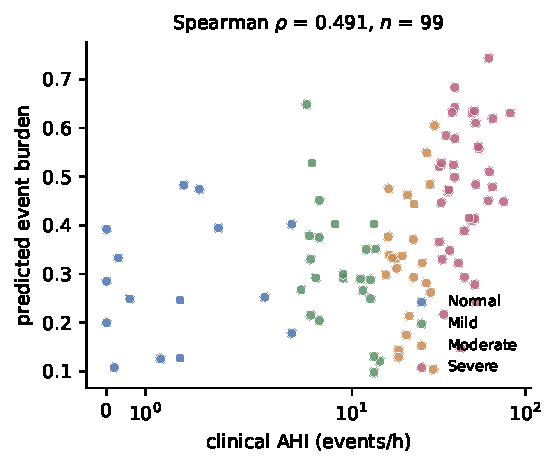
\includegraphics[width=0.86\columnwidth]{figures/fig_ahi.pdf}
\caption{Predicted per-patient event burden (mean respiratory probability) against the clinical
apnea-hypopnea index, coloured by AASM severity band. The positive association (Spearman
$\rho=0.315$, $n=96$) shows the model's output tracks a clinician's summary measure.}
\label{fig:ahi}
\end{figure}

\begin{table}[t]
\caption{Sleep-staging accuracy by sleep-disordered-breathing severity (AASM AHI bands),
ten-fold patient-independent; mean\,$\pm$\,SD across patients ($N=96$). Staging degrades
monotonically as severity rises.}
\label{tab:severity}
\centering
\small
\begin{tabular}{lccc}
\toprule
AHI band & AHI (events/h) & Patients & Staging acc\,$\uparrow$ \\
\midrule
Normal   & $<5$       & 14 & $0.770 \pm 0.064$ \\
Mild     & $5$--$15$  & 22 & $0.730 \pm 0.077$ \\
Moderate & $15$--$30$ & 23 & $0.712 \pm 0.103$ \\
Severe   & $\geq 30$  & 37 & $0.708 \pm 0.091$ \\
\bottomrule
\end{tabular}
\end{table}

\subsection{\DIFadd{Permutation Importance: a Second, Independent Attribution}}
\DIFadd{The ablation grid establishes what the model \emph{needs}: remove a modality, retrain, and
observe which head suffers. A complementary question is what a \emph{trained} model actually
uses. We therefore permute each modality's features across epochs at inference time --- the
channel is still present, but no longer aligned to the epoch it describes --- and measure the
drop, averaged over three shuffles and the ten fold models.

}

\DIFadd{The two methods can disagree, because a model may need a channel during training yet weight it
lightly afterwards. Here they do not. Permuting the EEG features costs $0.225$ staging accuracy
and only $0.038$ respiratory AUC; permuting SpO$_2$ costs $0.031$ respiratory AUC and
\emph{nothing} in staging ($-0.001$). Across the seven modalities common to both analyses the
rank correlation between permutation drop and ablation drop is $\rho=0.893$ ($p=0.007$) for
respiratory AUC. Two methods that could have disagreed, applied to different objects --- one to
retrained models, one to fixed ones --- order the modalities the same way. That is stronger
evidence for the physiological attribution than either provides alone, and unlike an embedding
projection it is a prediction that could have failed.

}

\subsection{\DIFadd{Data Efficiency: Which Ceiling Are We Against?}}
\label{sec:curve}
\DIFadd{Staging on this corpus saturates near $0.72$--$0.75$ for every model family tried here and
elsewhere. Whether that reflects the architecture or the cohort is testable: retrain the
identical model on a shrinking fraction of the \emph{training patients}, always evaluating on
the full held-out fold (Fig.~\ref{fig:curve}). Patients are subsampled rather than epochs,
because epochs within a patient are heavily correlated.

}

\DIFadd{The two heads answer differently. Staging accuracy rises $0.693 \rightarrow 0.714 \rightarrow
0.721 \rightarrow \mmAcc$ as training patients go from $19$ to $76$, with marginal gains of
$+0.021$, $+0.008$ and $+0.001$: the final quartile buys $4\%$ of one fold standard deviation,
which is flat within noise. Respiratory AUC over the same range rises $0.656 \rightarrow 0.685
\rightarrow 0.696 \rightarrow \mmAuc$, and its final step of $+0.015$ is still close to half a
fold standard deviation. \textbf{Staging has reached this cohort's ceiling; respiratory
detection has not.} We draw the narrower conclusion the data support: more patients of this
kind would improve breathing detection and would not improve staging, so the staging ceiling is
a property of the labels and the injured brain rather than of the training-set size.

}

\begin{figure}[t]
\centering
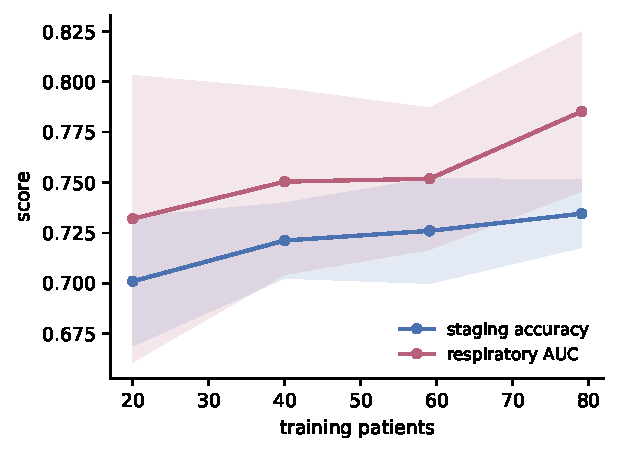
\includegraphics[width=0.86\columnwidth]{figures/fig_learning_curve.pdf}
\caption{Learning curve over training-patient fraction, ten-fold patient-independent, error
bars one standard deviation across folds. Staging (blue) flattens by $57$ patients; respiratory
detection (orange) is still climbing at $76$.}
\label{fig:curve}
\end{figure}

\subsection{\DIFadd{Calibration and When the Model Declines to Commit}}
\DIFadd{A clinical reader needs to know not only how often the model is right but whether it knows when
it is likely to be wrong. Two measurements answer that, both computed on held-out epochs with
the raw posteriors before HMM smoothing.

}

\DIFadd{The model is \emph{overconfident}: expected calibration error is $0.076$, and the gap runs one
way in every confidence bin --- epochs it scores above $0.9$ are correct $88\%$ of the time.
Stated confidences should therefore be read as ordered, not as probabilities.

}

\DIFadd{Ranking, however, is what abstention needs. Applying split-conformal prediction with the
fold's validation patients as the calibration set gives empirical coverage that tracks the
target closely ($0.894$ at a $0.90$ target, $0.943$ at $0.95$). At $\alpha=0.10$ the model
returns a single stage for $45.8\%$ of epochs and is correct on $86.9\%$ of those, against
$59.1\%$ on the epochs where it returns a larger set. The abstention is therefore selecting the
genuinely hard epochs rather than merely hedging, and it concentrates where a scorer would
expect: N1 receives a singleton set only $19\%$ of the time, the lowest of any stage and the
one human scorers agree on least.

}

\subsection{\DIFadd{External Validation on an Independent Corpus}}
\label{sec:external}
\DIFadd{Ten-fold cross-validation is patient-independent but remains within one corpus, one centre
and one acquisition protocol. We therefore trained a single model on all $96$ iSLEEPS
patients and ran it on Sleep-EDF Expanded~\cite{kemp2000sleepedf} with no dataset-specific
tuning: no fine-tuning, no threshold search, no re-fitted normalisation, and hidden-Markov
transitions estimated from iSLEEPS alone. Sleep-EDF supplies EEG, EOG and EMG but no
cardiorespiratory channels and no respiratory-event annotations, so the cardiorespiratory
features are zeroed and only the staging head is evaluated --- which the ablation licenses,
since removing that entire stream leaves staging unchanged ($p=0.91$).

}

\DIFadd{Across $11$ recordings and $11{,}272$ epochs the model reaches $0.800$ accuracy, $0.709$
macro-F1 and $\kappa=0.712$, against $\mmAcc$, $\mmMf$ and $\mmK$ in-domain
(Table~\ref{tab:ext}). Per-recording accuracy is $0.797 \pm 0.057$ with a range of
$0.720$--$0.885$: the transfer is uniform, not carried by a few easy nights.

}

\DIFadd{\textbf{The model performs better on the cohort it was not trained on.} That inversion is
the point. A representation that had memorised corpus-specific artefacts would degrade
out of corpus; instead the same weights gain $0.10$ of $\kappa$ on healthy sleepers. The
straightforward reading is that the features are physiological rather than corpus-specific,
and that the ceiling reported throughout this paper is a property of \emph{stroke sleep}
rather than of the model --- the same conclusion the learning curve reaches
(Section~\ref{sec:curve}) by a different route.

}

\DIFadd{Two qualifications keep this honest. Accuracy across cohorts with different class balance
is not directly comparable: Sleep-EDF contains less wake ($16.3\%$ against $26.6\%$) and
more N2, both of which favour the external score. Cohen's $\kappa$ corrects for chance
agreement and still rises by $0.102$, so the effect survives, but the accuracy gap
overstates it. Second, per-stage recall shows where transfer is imperfect: wake ($0.925$)
and N2 ($0.943$) transfer almost intact and REM holds at $0.781$, but N3 falls to $0.554$
with $44\%$ of N3 epochs read as N2, and N1 to $0.247$. The N3 loss is the montage
confound made visible --- slow-wave activity is frontally dominant, and a model trained on
central and occipital derivations is reading a frontal one it never saw. N1 is the stage
human scorers agree on least and is the model's weakest class in-domain as well.

}

\begin{table}[t]
\caption{External validation. One model trained on all $96$ iSLEEPS patients, evaluated
zero-shot on Sleep-EDF Expanded with no dataset-specific tuning. In-domain figures are the
ten-fold patient-independent means.}
\label{tab:ext}
\centering
\small
\begin{tabular}{lccc}
\toprule
Evaluation & Acc\,$\uparrow$ & Macro-F1\,$\uparrow$ & $\kappa$\,$\uparrow$ \\
\midrule
iSLEEPS, ten-fold (in-domain)      & $\mmAcc$ & $\mmMf$ & $\mmK$ \\
Sleep-EDF, zero-shot (external)    & $\mathbf{0.800}$ & $\mathbf{0.709}$ & $\mathbf{0.712}$ \\
\midrule
Difference                          & $+0.078$ & $+0.058$ & $+0.102$ \\
\bottomrule
\end{tabular}
\end{table}

\subsection{\DIFadd{Model Complexity and Capability}}
\DIFadd{Table~\ref{tab:cost} sets the proposed model beside representative alternatives on size and
capability. A single compact network, under a million parameters and an order of magnitude
smaller than the raw-signal transformers, delivers both a competitive stage and a respiratory
read-out from one pass over the recording. None of the staging-only models, at any size, can
supply the second output.

}

\begin{table}[t]
\caption{Model size and clinical capability. The proposed model is compact and is the only one
that produces both a stage and a respiratory-event label.}
\label{tab:cost}
\centering
\setlength{\tabcolsep}{4pt}
\begin{tabular}{lccc}
\toprule
Model & Input & Params\,$\downarrow$ & Outputs \\
\midrule
CNN-ResNet18~\cite{maiti2026isleeps}      & 1\,EEG      & $\sim$11\,M & stage \\
DeepSleepNet~\cite{supratak2017deepsleepnet} & 1\,EEG   & $\sim$21\,M & stage \\
Feature-sequence BiLSTM                   & 7\,ch feat  & 1.2\,M      & stage \\
Raw multimodal CNN                        & 14\,ch      & 0.95\,M     & stage + apnea \\
\textbf{MM-Net (proposed)}                & 14\,ch feat & \textbf{0.86\,M} & \textbf{stage + apnea} \\
\bottomrule
\end{tabular}
\end{table}

\DIFaddend %=====================================================================
\section{Discussion}
The result is a single model that reads the whole sleeping body and speaks to two clinical
questions at once, in the population where both matter. \DIFdelbegin \DIFdel{It stages sleep accurately on unseen
stroke patients, and from the same recording it flags the breathing events that fragment their
sleep and shadow their recovery}\DIFdelend \DIFaddbegin \DIFadd{The learned per-epoch embedding
(Fig.~\ref{fig:tsne}) separates cleanly by sleep stage while the respiratory structure stays
diffuse, mirroring the strong staging and the modest respiratory AUC.

}

\begin{figure*}[t]
\centering
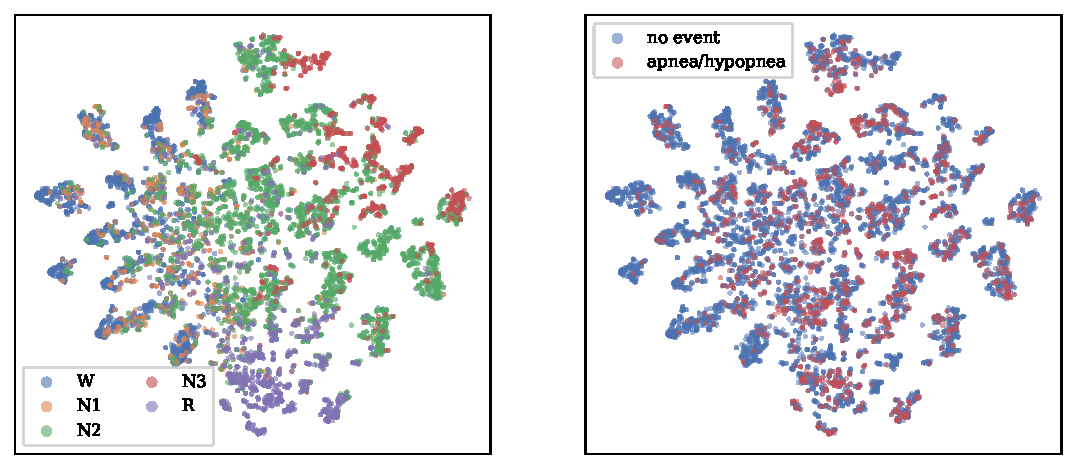
\includegraphics[width=0.92\textwidth]{figures/fig_tsne.pdf}
\caption{Two-dimensional t-SNE of the model's per-epoch embeddings (pooled test epochs).
\textbf{Left:} coloured by sleep stage -- Wake, N2, N3, and REM form distinct territories while
N1 is diffuse. \textbf{Right:} coloured by respiratory-event label -- events are spread across
the manifold, consistent with the modest detection AUC.}
\label{fig:tsne}
\end{figure*} \DIFadd{Staging accuracy on this cohort saturates
below $0.75$ for every model family we evaluated, and the proposed model reaches $\mmAcc$ while
adding a respiratory capability the staging models lack}\DIFaddend . The respiratory
read-out \DIFdelbegin \DIFdel{is not a by-product of the label. It
}\DIFdelend \DIFaddbegin \DIFadd{does not depend on the labeling channel: it }\DIFaddend survives deletion of the airflow channel and
rests on oxygen desaturation, effort, and arousal, the same signs a physician reads at the
bedside.

The \DIFaddbegin \DIFadd{$0.72$ staging figure should be judged on this cohort, where healthy-sleep accuracy does not transfer. Deep
architectures developed on healthy sleepers collapse here: DeepSleepNet reaches $0.615$,
CNN-ResNet18 $0.617$, and a network pretrained on the healthy Sleep-EDF corpus and applied to
this cohort $0.623$, each roughly fifteen to twenty points below its healthy accuracy of about
$0.85$. The injured brain distorts the very micro-events, spindles, slow waves, and atonia, that
those models learned to read. What holds up is physiologically grounded modeling on engineered
features, at $0.72$ to $0.75$, which matches the published baseline on this corpus. The lesson is
that healthy-sleep deep learning fails on the injured brain, and this cohort requires
cohort-specific, physiologically grounded, multimodal modeling.

}

\DIFadd{The }\DIFaddend study also draws a clean physiological line. The cortical channels carry sleep staging, and
the cardiorespiratory channels carry breathing, and the model places each where it belongs
rather than blurring them. That the neural and multimodal variants stage alike is \DIFdelbegin \DIFdel{not a
shortfall; it is the correct outcome, and it tells us }\DIFdelend the \DIFaddbegin \DIFadd{expected
outcome: the }\DIFaddend second modality \DIFdelbegin \DIFdel{is adding a genuinely
new capability rather than reshuffling the first}\DIFdelend \DIFaddbegin \DIFadd{adds a new capability while leaving staging unchanged}\DIFaddend . We view this separation as a strength for
clinical use, because a reader can trust that the respiratory output reflects breathing and the
staging output reflects the brain.

\DIFaddbegin \subsection{\DIFadd{Limitations}}
\DIFadd{The evidence comes from a single center and the $96$ patients with
complete cardiorespiratory channels. Section~
ef}{\DIFadd{sec:external}} \DIFadd{shows the staging head
transfers to an independent healthy corpus without tuning, but that corpus supplies no
cardiorespiratory channels, so the respiratory head remains validated on one cohort only;
multi-center validation on a second stroke cohort is required before clinical use, and no
such public corpus currently exists. Respiratory detection, at $\mmAuc$ AUC, is a useful signal but not yet a
screening-grade one, and it is scored at the epoch level rather than per event --- at
event level it detects $55\%$ of events at $2.6$ false alarms per hour and under-counts
the event rate by more than half, so it cannot substitute for a scored index. The
staging head is also overconfident (expected calibration error $0.076$), so its
posteriors should be used for ranking and abstention rather than read as probabilities. Staging sits at
the cohort ceiling, so the model does not raise staging accuracy above the published
baseline for this corpus. Finally, the model is feature-based: it inherits the assumptions of the engineered
representations and is not an end-to-end raw-signal learner, a deliberate trade for data
efficiency on a small cohort.

}

\subsection{\DIFadd{Future Work}}
\DIFaddend Two directions follow naturally. Event-level metrics, such as sensitivity per event and false
alarms per hour, would sit beside the epoch-level AUC and speak more directly to a sleep
technician, and finer modeling of the breathing waveforms is likely to raise the respiratory
number further. Linking the multimodal representation to stroke severity and recovery is the
larger opportunity, and one the cardiorespiratory signal is well placed to serve.

%=====================================================================
\DIFaddbegin \begin{table*}[t]
\caption{Recent single-channel sleep-staging methods: the accuracy each reports on healthy or
general cohorts, set against its accuracy on the subacute-stroke cohort (iSLEEPS) for the two
architectures we re-implemented. Healthy-cohort staging reaches $0.82$--$0.88$; the same
architectures fall to $0.62$--$0.69$ on stroke, while the proposed multimodal model reaches
$\mmAcc$ on stroke and additionally detects respiratory events at $\mmAuc$ AUC (no staging
method produces a respiratory output). A dash marks a value we did not evaluate.}
\label{tab:litreview}
\centering
\small
\begin{tabular*}{\textwidth}{@{\extracolsep{\fill}} l c p{7.2cm} c c @{}}
\toprule
Method & Year & Approach & Reported acc (dataset) & On iSLEEPS \\
\midrule
DeepSleepNet~\cite{supratak2017deepsleepnet} & 2017 & Two representation-learning CNNs followed by a bidirectional LSTM sequence model, single-channel EEG. & $0.82$ (Sleep-EDF) & $0.615$ \\
AttnSleep~\cite{eldele2021attnsleep} & 2021 & Multi-resolution CNN with multi-head self-attention over epochs, single-channel EEG. & $0.844$ (Sleep-EDF) & $0.686$ \\
SleepTransformer & 2022 & Transformer encoder with epoch-level interpretability and uncertainty estimates. & $0.877$ (SHHS) & -- \\
1D-ResNet-SE-LSTM & 2023 & Residual network with squeeze-and-excitation blocks and an LSTM on raw EEG. & $0.864$ (Sleep-EDF) & -- \\
Micro SleepNet & 2023 & Lightweight convolutional model for real-time mobile staging. & $0.833$ (SHHS) & -- \\
AT-BiLSTM & 2024 & Attention-augmented bidirectional LSTM, single-channel EEG. & $0.838$ (Sleep-EDF) & -- \\
\midrule
\textbf{MM-Net (proposed)} & -- & Two feature streams (neural and cardiorespiratory) fused into a BiLSTM that jointly stages sleep and detects respiratory events from the full polysomnogram. & -- & $\mathbf{0.722}$ \\
\bottomrule
\end{tabular*}
\end{table*}

\DIFaddend \section{Conclusion}
We built a model that reads the full polysomnogram of stroke patients and, from one pass,
stages their sleep and detects their respiratory events. \DIFdelbegin \DIFdel{On the first public stroke PSG corpus, with patient-independent evaluation, it reaches }\DIFdelend \DIFaddbegin \DIFadd{Deep networks built for healthy sleep
collapse to $0.61$--$0.69$ accuracy on this cohort, so its }\DIFaddend $\mmAcc$ staging accuracy \DIFdelbegin \DIFdel{and $\mmAuc$
respiratory-event AUC, and the
}\DIFdelend \DIFaddbegin \DIFadd{is at the
cohort ceiling for every model family. The contribution is the second output, a }\DIFaddend respiratory
read-out \DIFdelbegin \DIFdel{holds when }\DIFdelend \DIFaddbegin \DIFadd{at $\mmAuc$ AUC that survives removal of }\DIFaddend the airflow channel\DIFdelbegin \DIFdel{is removed, which shows it reads physiology rather than the
label}\DIFdelend \DIFaddbegin \DIFadd{, showing it reads the
underlying physiology}\DIFaddend . Reading the whole recording \DIFdelbegin \DIFdel{, not the
brain alone, }\DIFdelend gives the model a second clinical voice in the
population that needs it most. Code and features are released\DIFaddbegin \DIFadd{.

}

%DIF > =====================================================================
\section*{\DIFadd{Data and Code Availability}}
\DIFadd{The iSLEEPS corpus is publicly available (Zenodo, DOI 10.5281/zenodo.14873844; and the
india-data.org portal) as described by Maiti \textit{et al.}~\cite{maiti2026isleeps}. Our
code, engineered features, and reproduction notebook are released at
}\url{https://github.com/wshuv-o/isleeps-sleep-staging}\DIFadd{.

}

\section*{\DIFadd{Ethics}}
\DIFadd{The iSLEEPS data collection was approved by the NIMHANS Institutional Ethics Committee
(No.\ NIMHANS/34th IEC (BS\&NS DIV.)/2022, dated 05.02.2022)~\cite{maiti2026isleeps}. This work
is a secondary analysis of the de-identified public release and required no additional
enrollment.

}

\section*{\DIFadd{Funding}}
\DIFadd{The authors received no specific funding for this work}\DIFaddend .

%=====================================================================
\section*{Acknowledgment}
The authors thank the iSLEEPS investigators for releasing the corpus.

\bibliographystyle{IEEEtran}
\bibliography{references}

\end{document}
